\documentclass[a4paper,14pt, openany, twoside, draft]{extbook} % computer modern font calls
%\usepackage{fancybox}

\usepackage[final]{graphicx}
\graphicspath{{./pics/}{./paropt/pics/}}
\usepackage[usenames]{xcolor}
\usepackage[final]{minted}
%\usemintedstyle{emacs}
\usemintedstyle{tango}
%\usemintedstyle{trac} % better (more bold faces}
%\usemintedstyle{manni} % pastel colors
%\usemintedstyle{bw}
\definecolor{mintedbg}{rgb}{0.95,0.95,0.95}
\setminted{breaklines=true,fontsize=\small,funcnamehighlighting=true,python3=true}

%\newminted{prolog}
\protect\newminted[proexp]{prolog}{style=bw}

% Main style definition
% ---------------------
% ISU standard handbook.
%\usepackage[times,fancybot,firamono]{subook} % looks less good than inconsolata
\usepackage[times,fancybot,inconsolata]{subook} % Looks Good
%\usepackage[times]{subook}

% Заменить в коде кой-что на математические формулы
% http://www.tug.org/texlive/Contents/live/texmf-dist/doc/latex/base/alltt.pdf

% Требования к оформлению Типографии ИГУ
% http://lawinstitut.ru/ru/about/services/izdatelstvo/trebovaniya.html
%

% ISU standard monograph (less restrictive and more artistic)
% \usepackage[monograph,mag,times,smalltitles,fancybot,listbib,ptfonts,microtyping]{subook}

% Some artistism for monograph
% ----------------------------
%\makeatletter{}
%\renewcommand\su@chapter@font{\sffamily\sfcpshape\bfseries}
%\renewcommand\su@chapter@font@size{\LARGE}
%\makeatother{}
%\floatname{algorithm}{Процедура}
%\renewcommand{\listalgorithmname}{Список процедур}
%\renewcommand\cftsecnumwidth{5ex}
%\tolerance=5000
%\renewcommand{\chaptername}{Глава}
%\usepackage[final]{hyperref}

\definecolor{mygreen}{rgb}{0,0.6,0}
\definecolor{mygray}{rgb}{0.5,0.5,0.5}
\definecolor{mymauve}{rgb}{0.58,0,0.82}


\usepackage{tikz}
\usetikzlibrary{arrows,arrows.meta,shapes}
\usetikzlibrary{shadows}
\newcommand*\keystroke[1]{%
  \tikz[baseline=(key.base)]
    \node[%
      draw,
      fill=white,
      drop shadow={shadow xshift=0.25ex,shadow yshift=-0.25ex,fill=black,opacity=0.75},
      rectangle,
      rounded corners=4pt,
      inner sep=1pt,
      line width=0.7pt,
      font=\footnotesize\sffamily
    ](key) {~#1~\strut}%
  ;%
}

\long\def\rem#1{}
%\def\AR{{\em Прим.~авторов~пособия}}
\def\emphbib#1{#1}
\newenvironment{questions}{\subsubsection*{Вопросы для самопроверки}\begin{enumerate}\itemsep0pt minus 0.3pt\parskip0pt plus 0.3pt}{\end{enumerate}}

\newtheorem{example}{Пример}[chapter]
\hypersetup{
    bookmarks=true,         % show bookmarks bar?
    unicode=true,           % non-Latin characters in Acrobat’s bookmarks
    pdftoolbar=true,        % show Acrobat’s toolbar?
    pdfmenubar=true,        % show Acrobat’s menu?
    pdffitwindow=false,     % window fit to page when opened
    pdfstartview={FitH},    % fits the width of the page to the window
    pdftitle={Компьютерные науки, часть 4},    % title
    pdfauthor={Евгений Александрович Черкашин},     % author
    pdfsubject={Методическое пособие},   % subject of the document
    pdfcreator={EMACS-24.4:AuCTeX},   % creator of the document
    pdfproducer={LuaLaTeX}, % producer of the document
    pdfkeywords={Искусственный интеллект} {Логическое
      программирование} {Планирование действий} {Удовлетворение
      ограничений} {Генетическое программирование} {Имитационное моделирование}, % list of keywords
    pdfnewwindow=true,      % links in new window
    colorlinks=true,       % false: boxed links; true: colored links
    linkcolor=[rgb]{0 0.4 0.1},          % color of internal links (black)
    citecolor=blue,        % color of links to bibliography
    filecolor=black,      % color of file links
    urlcolor=[rgb]{0.3 0.0 0.3}           % color of external links
}

%\renewcommand{\headrulewidth}{1pt}

\clubpenalty=3000
\widowpenalty=3000
%\brokenpenalty=10000
%\floatingpenalty=10000

%% \setdefaultlanguage{russian}
%% \setmainlanguage{russian}
%% \setotherlanguage{english}

%\newenvironment{mygroup}{}{}

\renewcommand\baselinestretch{1.5} % FIXME Какой интервал тут реально получится?
\newcommand{\eeng}[1]{\emph{\foreignlanguage{english}{#1}}}

\definecolor{rclr}{rgb}{0.5,0.1,0.1}
\definecolor{eclr}{rgb}{0,0.5,0.5}
\colorlet{acolor}{blue}
\colorlet{rcolor}{red}
\definecolor{ncolor}{rgb}{0.5,0.5,0.1}
\newcommand{\aaa}[2][acolor]{\noindent\textcolor{eclr}%
{+\ [}\textcolor{#1}{#2}\textcolor{eclr}{]}}
\newcommand{\rrr}[2][rcolor]{\noindent%
\textcolor{eclr}{-\ [}\textcolor{#1}{#2}\textcolor{eclr}{]}}
\newcommand{\nnn}[2][ncolor]{\noindent%
\textcolor{eclr}{!\ [}\textcolor{#1}{#2}\textcolor{eclr}{]}}
\newcommand{\goforth}[1]{$\,\hookrightarrow$\pageref{#1}}

% \begin{figure}
%   \centering
%   \def\svgwidth{\columnwidth}
%   \includesvg{image}
% \end{figure}

\parskip=0pt plus 0.3pt
\begin{document}
% \itemsep3pt plus 0pt minus 3pt
% \widowpenalty=10000
% \clubpenalty=10000
% \renewcommand\sutitlefontface{\Large\ptsans\nwshape\bfseries}
% \theorembodyfont{\rmfamily}

%\lstset{language=Prolog, morecomment=[l]{\%}}
\renewcommand{\chaptername}{} % for ISU Handbooks
\renewcommand{\refname}{Рекомендуемая литература} % ... also
\renewcommand{\bibname}{\refname}
\begin{titlepage}
\thispagestyle{empty}
%\aaa{Эта и следующая страница вставляется из .docx}
\begin{center}{\small{}
Министерство образования и науки
Российской Федерации \\
Федеральное государственное бюджетное образовательное\\
учреждение высшего профессионального образования\\
<<Иркутский государственный университет>> \\
Институт математики, экономики и информатики
%\\[2ex]
%    Учреждение Российской академии наук \\
%<<Институт динамики систем и теории управления \\
%Сибирского отделения РАН>>
}
\vfill
%\hbox to \linewidth{\hfill\bfseries Е.~А.~Черкашин\hfill}
 \vspace{2em}
{\large\bfseries КОМПЬЮТЕРНЫЕ НАУКИ\\В четырех частях\\Часть 4\\}
 \vspace{2em}
{Учебное пособие}
\vfill
%\vfill
\vfill
 \textbf{Иркутск 2014}
\end{center}
\end{titlepage}
%\newpage
%\begingroup
%\normalfont \ttfamily Это \textbf{текст} в \itshape нормальном \bfseries фонте\sffamily етноф\nwshape фонт\rmcpshape тноф\sfcpshape фонт\ttfamily тноф...
%\endgroup

\newpage
\begin{mygroup}
\thispagestyle{empty}
\noindent УДК 681.3.06 (075.8)\\ % (075.8) = Handbook
% \noindent УДК~165:681.3.06+62-52\\
\noindent ББК 32.97я73\\
% ББК 87.4:32.973-01+32.813\\ % monograph
\noindent\mbox{}\hspace{2em}К63
\begin{center}\small
Печатается по решению ученого совета ИМЭИ\\[2ex]
\bfseries Издание выходит в рамках Программы\\
стратегического развития ФГБОУ ВПО <<ИГУ>>\\
на 2012--2016 гг., проект Р121-02-001
\end{center}
\vspace{0.5ex}
\begin{center}\small
  \textbf{Рецензенты:} \\
  %канд.~техн.~наук~{\em В.~С.~Ульянов},\\ канд.~физ.-мат.~наук~{\em А.~А.~Лемперт}\\
  \textbf{Авторы:}\\
  Л.~В.~Рожина (часть 1 глава 1"=5), А.~А.~Ветров (приложения к части 1),\\
  А.~Е.~Хмельнов (часть 2), Р.~К.~Фёдоров (часть 3), Е.~А.~Черкашин (часть 4)
\end{center}
\vfill
\noindent\begin{minipage}[t]{2em}
\noindent\mbox{}\\
К63
\end{minipage}%
\begin{minipage}[t]{0.95\linewidth}
\setlength{\parindent}{5ex}
\noindent{\bfseries Черкашин~Е.~А.}

Компьютерные науки~4\,{}: учеб.~пособие\,/~Е.~А.~Черкашин, Л.В. Рожина,Р.К. Фёдоров, А.Е. Хмельнов, А.А. Ветров..~-- Иркутск\,: Изд-во ИГУ, 2014.~-- \pageref{lastpage}~c.

{\bfseries ISBN 978-5-9624-0938-2}
\vspace{2ex}

\begingroup\footnotesize\parskip0pt
\vspace{1ex}


Четвертая часть учебного пособия включает разделы: информация и данные, вычислительная система, устройство персонального компьютера, системное и прикладное программное обеспечение, компьютерные сети, вторая~---  программирование, третья~--- базы данных и СУБД, четвёртая~--- системы искусственного интеллекта.

Предназначено для студентов вузов, обучающихся по направлениям «Математика», «Прикладная математика и информатика», «Математическое обеспечение и администрирование информационных систем», «Информационная безопасность».

%Библиогр. 11 назв. Ил. 24.

%В пособии представлены лекционные материалы и лабораторные работы курса <<Рекурсивно"=логическое программирование>>: базовые термины искусственного интеллекта, задачи, методы и их свойства; основы рекурсивно"=логического программирования на языке Пролог; типичные задачи, решение которых лаконично представляется как рекурсивные и переборные алгоритмы. Пособие содержит задания на лабораторный практикум по темам <<Формализация>>, <<Обработка списков>>, <<Метод Британского музея (отобразить и проверить)>> и <<Базы данных>>.

%Пособие предназначено для студентов специальности <<инженер"=программист>>, <<инженер\,---\,системный программист>>. Изучение материала будет полезно студентами других специальностей, так или иначе связанных с программированием, формальной логикой и комбинаторикой.

\mbox{}
\endgroup
\end{minipage}
\mbox{}\hspace{0.7\linewidth}
\begin{minipage}{0.3\linewidth}\small
\noindent УДК 681.3.06 (075.8)\\
\noindent ББК 32.97я73
\end{minipage}

\vfill
\noindent\begin{minipage}[t]{0.35\linewidth}\small
\noindent ISBN 978-5-9624-0938-2
\end{minipage}%
\begin{minipage}[t]{0.65\linewidth}\small
\begin{itemize}
\setlength{\itemsep}{-0.5ex}
\setlength{\parsep}{0pt}
\item[\copyright{}] Черкашин~Е.~А., 2014
\item[\copyright{}] ФГБОУ ВПО <<ИГУ>>, 2014
%\item[\copyright{}] Институт динамики систем и теории управления СО РАН, 2014
\end{itemize}
\end{minipage}
\end{mygroup}
\clearpage
%\setcounter{page}{2}
\tableofcontents
\clearpage

\newpage
\chapter*{Предисловие}

%\nnn{Переписать предисловие на последнем этапе.}

% $$
% \int\limits_1^1f(x)dx.
% $$

Интерес математиков к решению сложных задач при помощи вычислительной техники постоянно возрастает.  Разрабатываются программные пакеты автоматизации выполнения математических операций и даже решения стандартных задач в автоматическом режиме.  Алгоритмы, реализованные в таких пакетах, используют современные и классические методы поиска решения.  Решение представляется в виде комбинации различных вариантов преобразования сложных структур данных, входных и выходных переменных различных методов.  Для того чтобы продуктивно пользоваться этими пакетами, необходимо изучать, как они работают, как получают требуемое решение.

В учебном пособии в форме тренинга (\eeng{tutorial}) представляются самые простые методики поиска решения дискретных задач, относящихся к различным классам искусственного интеллекта (ИИ) <<логическое программирование>>, <<планирование действий>>, <<решение задач в терминах ограничений>> и <<символьные вычисления>> (<<компьютерная алгебра>>).  Основная задача пособия состоит в выработке навыков автоматизации некоторых аспектов творческой деятельности математика при помощи вычислительных машин и классических средств реализации программ из области ИИ.  Навыки решения таких задач позволят в будущем создавать собственные программные системы, реализующие новые методы, для которых еще не было разработано соответствующего программного обеспечения.

Пособие разработано для студентов, обучающихся по специальности <<Математика>>, может быть использовано всеми заинтересованными программистами, желающими овладеть некоторыми методами искусственного интеллекта. Пособие включает подборку материала по курсам <<Рекурсивно"=логическое программирование>>, <<Искусственный интеллект>>. Оно никоим образом не претендует на полноту излагаемого материала и базируется на личном опыте преподавания. Пособие следует воспринимать как путеводитель, и учащиеся в процессе обучения должны активно использовать литературу, на которую в тексте указаны ссылки. В цитируемом тексте в виде сносок авторы позволяют себе высказывать свое отношение к изложенному.

Форма тренинга, примененная в пособии, позволяет рассматривать материал в процессе монолога с читателем.  Ставится задача, обсуждаются возможные варианты ее решения.  Затем рассматривается новый материал, необходимый для реализации выбранного решения.  Если в процессе появляется необходимость в изучении дополнительного материала, то параллельно основному монологу создается новый.  Если читатель знаком с излагаемым материалом, то его можно пропустить и перейти далее (по ссылке) к рассмотрению решения задачи.  Форма изложения, принятая в пособии, предполагает, что материал осваивается с самого начала до самого конца.  То есть эту книгу будет сложно использовать как справочник.

Практически все разделы пособия представляют собой авторскую разработку, за исключением вводной части, которая содержит компиляцию материала из различных справочников.  Во всем тексте, по возможности, указаны ссылки на оригинальные источники информации.  Авторы не преследуют целью коммерческое использование учебного пособия.  В его электронной версии ссылки на литературу в списке литературы~--- активные и ведут к найденным в Интернете электронным версиям книг.  Читатель должен решать самостоятельно: скачивать их из Интернета, покупать в магазинах или искать в библиотеках.

Данное учебное пособие является свободной книгой (так же как и свободное программное обеспечение), которую можно при определенных условиях читать, копировать и дополнять новым материалом. Адрес исходного кода методического пособия: \url{https://github.com/eugeneai/ais/tree/clean-isu}. Исходный код разрешено использовать в соответствии с лицензией \foreignlanguage{english}{CC BY-NC-SA 4.0 (Attribution-NonCommercial-ShareAlike 4.0 International)}, которая позволяет включать материал в свои произведения (необходимо указывать автора оригинальных материалов), запрещает коммерческое использование материалов (ввиду наличия заимствований в первой части) и требует распространение производных материалов производить по этой же самой лицензии (по указанной выше же причине). Адрес лицензии: \url{http://creativecommons.org/licenses/by-nc-sa/4.0/}.

В тексте пособия использована следующая разметка:
\begin{description}
\item[\normalfont{\tt моноширинным шрифтом}] приводятся программы, отрывки программ в основном тексте пособия, а также имена идентификаторов, т.~е. все, что имеет какое"=либо отношение к тексту программы;
\item[\normalfont{\em наклонным шрифтом}] выделяются новые термины, вводимые в текст и возникающие, например, в определениях, а также текст выделенных примеров;
\item[\normalfont при помощи <<кавычек>>] выделяются метафоры, значения, элементы текстов программ, цитаты, слова, использованные в переносном смысле, и т.~д.
%\item[\normalfont{\sf Рубленым шрифтом}] декорируются тексты, которые надо как-то особо выделить на общем фоне.
\end{description}

Авторы пособия надеются, что материал, представленный в данной книге, будет полезным при решении практических и научных задач, а также что он вызовет интерес студента к разработке программного обеспечения в области искусственного интеллекта.

%\aaa{Thenks To Seseg.}

\medskip

\noindent\hbox to \linewidth{\hfill\sf От имени и по поручению коллектива авторов,}
\noindent\hbox to \linewidth{\hfill\sf доцент кафедры ИТ ИМЭИ ИГУ}
\noindent\hbox to \linewidth{\hfill\sf канд.~техн.~наук Е.~А.~Черкашин}

\vfill
\makeatletter
\noindent{\sf P.~S.} Авторов искать по адресу \href{mailto:eugeneai@icc.ru}{\tt{}eugeneai@icc.ru}, в поле <<{\tt тема}>> просим указывать <<ИИ-2014>>.
\makeatother

\chapter{Информатика и искусственный интеллект}

Среди задач, которые решают современные программисты, выделяются задачи создания программных систем математического моделирования и прогнозирования, проектирования и реализации информационных систем и баз данных, системного программного обеспечения. Все перечисленные задачи объединяет одно общее свойство~--- для широкого практического класса задач можно построить детерминированную процедуру (например, алгоритм) их решения. Существует большой класс задач, для которых такую процедуру построить достаточно сложно, а порой и невозможно. Например, разработать игровую систему, способную играть в шахматы с человеком на высоком профессиональном уровне. К таким задачам относятся также и задачи поиска решения (планирование действий, или Problem Solving), распознавание образов, экспертные консультации, интеллектуальное управление сложными динамическими объектами и т.~д. В каждой такой задаче четко вырисовывается их первое общее свойство~--- необходимость {\em автоматизации принятия некоторого решения}. В других задачах четко вырисовывается еще одно свойство~--- {\em обработка символьной информации}. Примерами задач, обработка информации в которых основывается на преобразовании строк символов, выступают следующие задачи: автоматический перевод текста с одного естественного языка на другой, автоматическое доказательство теорем. В той или иной мере оба выделенных свойства присутствуют в каждой из перечисленных задач.

Средства искусственного интеллекта\footnote{В англоязычной литературе данный термин называется \emph{Artifical Inelligence, AI}.}, в частности логическое программирование, позволяет представить решение таких задач, алгоритм, в рекурсивном виде или в виде некоторого переборного процесса. Такое представление обладает одним полезным свойством~--- оно компактно и достаточно близко к исходной математической модели задачи по сравнению с изученной ранее процедурной парадигмой программирования. Программисту не требуется определять все действия, необходимые для достижения результата. Как правило, достаточно рассказать транслятору, какие данные есть в наличии, объяснить, как они связаны друг с другом и постановкой задачи. Система постарается получить решение самостоятельно. Логическое программирование прежде всего направлено на решение задач ИИ, поэтому в данном учебном пособии необходимо ввести читателя в базовые концепции ИИ. Для начала рассмотрим, как можно определить, относится ли ваша задача к задачам ИИ.

Рассмотрим задачи планирования действий. Что есть решение в этих задачах? Это ответ на вопрос <<Какие действия необходимо выполнить и в каком порядке их надо выполнять, чтобы достичь цели из некоторого начального состояния?>>. Получается, что ответ на этот вопрос есть некоторая конечная последовательность действий. Эта последовательность представляется в памяти компьютера в виде некоторого ряда чисел, кодирующего эту последовательность. Построить (найти) эту последовательность, выбрать последовательность из возможных альтернатив~--- это и есть принятие решения.

Есть еще один интересный аспект алгоритма~--- массовость, т.~е. алгоритмы должны строиться для некоторого класса задач, а не для конкретных входных данных. Что это значит? На вход программы, реализующей алгоритм, подаются какие"=либо входные данные, задающие конкретную задачу из класса решаемых алгоритмом задач. Теперь представим такую ситуацию, что на вход алгоритма невозможно подать все необходимые данные, т.~е. имеет место \emph{неполнота информации}. Или другой вариант: имеется два эксперимента с разными результатами, но с одинаковым набором исходных данных. Какие данные следует передавать на вход алгоритма? Этот случай связан с \emph{противоречивой информацией}. Разрабатывая программное обеспечение, позволяющее функционировать в таких условиях, приходится создавать подпрограммы, принимающие решение, что следует делать. Например, во втором случае можно запустить алгоритм для каждого набора данных и проанализировать полученные результаты. Может получиться так, что эти результаты не будут сильно отличаться друг от друга, а может этого не получиться. В последнем случае одним из вариантов дальнейших действий является поиск нового атрибута (характеристики), который позволит различать варианты, находящиеся в противоречии.

Задачи,  обладающие перечисленными свойствами, и методы их решения на ЭВМ в конечном счете составляют предмет исследования искусственного интеллекта~--- одного из разделов информатики (Computer Science).

\section{Определения}

В литературе можно найти целый спектр определений термина <<искусственный интеллект>>, однако, насколько известно авторам, ни один из них не принят как стандарт.

Среди многих точек зрения доминируют три \cite{AIDictionary}. Согласно первой, исследования в области искусственного интеллекта являются фундаментальными исследованиями, в рамках которых разрабатываются модели и методы решения задач, традиционно считавшихся интеллектуальными и не поддававшихся ранее формализации и автоматизации. Согласно второй точке зрения, новое направление связано с новыми идеями решения задач на ЭВМ, с разработкой принципиально иной технологии программирования, с переходом к архитектуре ЭВМ, отвергающей классическую архитектуру, которая восходит еще к первым ЭВМ. Наконец, третья точка зрения, по"=видимому, наиболее прагматическая, состоит в том, что в результате работ в области искусственного интеллекта рождается множество прикладных систем, решающих задачи, для которых ранее создаваемые системы были непригодны.

Достаточно простые определения {\em искусственного интеллекта} показаны в табл.~\ref{pic:determai} \cite{Russell}. Выделяются несколько комбинаций двух пар ключевых терминов: <<размышлять>> и <<вести себя>>, <<как человек>> и <<рационально>>.

\begin{table}[h]
\begin{center}
\caption{Несколько определений искусственного интеллекта} \label{pic:determai}%
\begin{tabular}{|p{0.45\linewidth}|p{0.45\linewidth}|}
 \hline
   Системы, которые размышляют, как люди
 &
   Системы, которые размышляют рационально
 \\ \hline
   Системы, которые ведут себя, как люди
 &
   Системы, которые ведут себя рационально
 \\  \hline
\end{tabular}
\end{center}
\end{table}

{\em Искусственный интеллект} как наука насчитывает уже около 60 лет. Задачей этой науки является воссоздание с помощью искусственных устройств (в основном с помощью ЭВМ) разумных рассуждений и действий \cite{Lauriere}.

{\em Искусственный интеллект}~--- раздел информатики, изучающий методы, способы и приемы моделирования и воспроизведения с помощью ЭВМ разумной деятельности человека, связанной с решением задач \cite{math_slov:88}.

\subsection{Тест Тьюринга}

В книге \cite{Russell} вводится понятие {\em агента}. {\em Агент}~--- субъект, находящийся в среде, имеющий цель своего существования, взаимодействующий со средой или другими агентами с помощью {\em рецепторов} и {\em эффекторов}. Рецепторы воспринимают информацию о среде, а эффекторы~--- это способ воздействия на среду, которое меняет среду, а следовательно, и информацию о среде. Агентом может являться как программа, так и человек. Вводится понятие {\em интеллектуального агента}~--- агента, обладающего интеллектом.

Агенты взаимодействуют друг с другом. Примером такого взаимодействия выступают, например, общение человека с человеком или работа человека с компьютерной программой.

Тест Тьюринга предложен Аланом Тьюрингом (1950) и был разработан, чтобы представить действующее определение интеллекта \cite{Russell}. Тьюринг определял интеллектное поведение как возможность достижения человеческого уровня производительности во всех задачах, где возможно обмануть человека, задающего вопросы. Грубо говоря, предложенный им тест состоял в следующем. Компьютеру задает вопросы человек через удаленное устройство. Тест считается пройденным, если человек не может сказать, кто или что на другом конце устройства: компьютер или человек.

С точки зрения агентов, этот тест можно представить так: один интеллектуальный агент (человек) по информационному каналу, не позволяющему ему использовать иную информацию, кроме ответов на поставленные им вопросы, анализирует поступающую информацию (ответы собеседника) от другого агента (испытуемого). Если первый агент не в силах определить, кто на другом конце информационного канала~--- человек или устройство, тогда считается, что испытуемый агент обладает интеллектуальными свойствами.

\subsection{Задачи ИИ}

Всякая задача, для которой неизвестен алгоритм решения, априорно относится к ИИ. Перечислим некоторые направления (задачи) ИИ \cite{AIDictionary}: \nnn{убрать отступ, добавить выступ}
\begin{description}
 \item [Восприятие и распознавание образов.] К таким задачам относятся распознавание текста (как печатного, так и рукописного), компьютерное зрение.
 \item [Автоматическое доказательство теорем.] В этом направлении решаются задачи  автоматизации математических исследований, разработки формальных (математических) методов логического вывода для поддержки решения других задач ИИ. Это направление нашло применение в задачах верификации программного и аппаратного обеспечения.
 \item [Игры.] Автоматизация решения игровых задач, например игры в шахматы, кал\'{а}х, реверси, а также других игр.
 \item [Решение задач (Problem Solving), планирование действий.] В этих задачах предполагается наличие некоторого выбора из возможных путей решения, требуется найти первое, лучшее или оптимальное решение. Примеры: составление расписания работы учебного учреждения, планирование действий автономного необитаемого аппарата.
 \item [Понимание естественного языка.] Как правило, системы понимания естественного языка являются составляющими информационных систем различного назначения: от автоматических систем заказа билетов до систем ввода экспертного знания.
 \item [Логическое программирование.] Языки и системы программирования  высокого выразительного уровня, построенные на основе результатов исследования формально"=логических систем, теорий исчислений. Эта область ИИ носит, кроме прочего, инструментальный характер, т.~е. логическое программирование является средством реализации систем ИИ.
 \item [Экспертные системы.] Экспертные системы  (ЭС) позволяют заменять человека"=эксперта в некоторой предметной области программной системой, способной проводить экспертные консультации пользователя. ЭС нашли широкое применение в индустрии.
 \item [Интеллектные информационные системы.] Эти cистемы объединяют разнородные интеллектные системы (например, системы речевого общения, решения задач и др.) для организации интеллектного доступа, обработки информации. Они, как правило, предназначены для работы с конечным пользователем низкой квалификации. Пример: электронные переводчики и разговорники.
 \item [Восприятие и усвоение знаний.] Одна из задач ИИ~--- это приобретение знаний\footnote{\emph{Англ.}~--- Knowledge Acquisition.} (обучение, наполнение базы знаний) от человека или самостоятельно из среды функционирования. Системы усвоения знаний используются как подсистемы других интеллектных систем.
 \item [Интеллектное управление \cite{Vass:2000}.] Новое направление, появившееся на стыке ИИ и теории управления, в котором разрабатываются управляющие системы, основанные на тех или иных методах ИИ. В настоящее время наиболее развиты методы управления на основе нечеткой логики и искусственных нейронных сетей. В этом новом направлении ведутся научные разработки Института динамики систем и теории управления СО РАН (\url{http://www.idstu.irk.ru}).
\item [Робототехника (Robotics).] Собирательное направление исследований, задачей которого является автоматизация функционирования роботов, вплоть до полной независимости их от человека.
\end{description}

\paragraph{Определение задач ИИ в контексте пособия.} К сфере искусственного интеллекта относятся задачи, обладающие следующими свойствами \cite{Lauriere}:
 \begin{itemize}
 \item в них используется информация в символьной форме: буквы, слова, знаки, рисунки. Это отличает область ИИ от областей, в которых традиционно компьютерам доверяется обработка данных в числовой форме\footnote{Например, математическое моделирование, базы данных.};
  \item в них предполагается наличие выбора; действительно, сказать, что не существует алгоритма\footnote{Интуитивное определение алгоритма: \emph{алгоритм}~--- это конечная последовательность действий, каждое из которых выполняется за конечное время, приводящая к определенному результату.},~--- это значит сказать, по сути дела, только то, что нужно сделать выбор между многими вариантами в условиях неопределенности, и этот недетерминизм, который носит фундаментальный характер, эта свобода действия являются существенной составляющей интеллекта.
 \end{itemize}

Излагаемый в пособии курс подразумевает непосредственное изучение технических аспектов применения методов ИИ, таких как применимость того или иного метода в конкретной задаче, реализация программных модулей конкретного метода. Поэтому в предлагаемом курсе мы будем использовать следующее определение искусственного интеллекта:
\begin{quote}{\em
Искусственный интеллект}~--- область информатики, в которой разрабатываются и исследуются методы построения программных систем и решения задач, так или иначе связанных с принятием решения и обработкой символьной информации\footnote{Данное определение задает термин в достаточно узком смысле.}.
\end{quote}

\subsection{Данные и знания}

Одним из фундаментальных терминов ИИ является термин {\em знание}. Данный термин также является сложным в смысле его конструктивного определения, понятного читателю. Как правило, авторы статей по ИИ сознательно уклоняются давать более или менее точные определения, предполагая, что читателю это уже известно.

Более формальный термин <<данные>> получил широкое распространение в научно"=техническом обиходе, в особенности в практике использования ЭВМ для решения самых разнообразных задач \cite{AIDictionary}. При этом вся обрабатываемая информация называется данными: начальными, промежуточными или конечными, входными или выходными. Для предложений естественного языка более привычны термин <<знание>> и глагол <<знать>>. Ни у кого не вызывает возражений использование этого слова в предложениях вроде <<Я знаю, как решить задачу>> или <<Я знаю, что вчера Петя встречался с Наташей>>. Сомнению может подвергаться лишь истинность подобных утверждений, но никак не возможность сочетания слова <<знать>> с фрагментами предложения, обозначающих любую информацию, о которой говорится, что она кому"=то известна.

Вопрос о разделении информации на данные и знания возник при разработке систем ИИ, определяемых в последнее время как системы, основанные на знаниях\footnote{На самом деле это определение не охватывает такую важную отрасль ИИ, как нейронные сети.}. Был предложен ряд определений, отражающих различные аспекты этих понятий, но касающихся скорее форм (см. раздел \ref{sec:knowlege_repr}) представления данных и знаний, правил их использования, чем их сути.

\subsubsection*{Два подхода к разработке методов и средств ИИ}
\begin{mygroup}
%\small\sf
\begin{description}
\item[<<Снизу вверх>>.] Суть подхода выражена в фразе <<{\em Давайте создадим механическое (вычислительное) устройство, похожее на (моделирующее) мозг человека, а затем посмотрим, как оно будет решать задачи ИИ}>>.
\item[<<Сверху вниз>>.] В основе этого подхода лежит {\em разработка методов моделирования процесса мышления человека (логических выводов, логических рассуждений)}.
\end{description}

Методы и системы ИИ, основанные на подходе <<Снизу вверх>>, как правило, представляют собой сложную сеть взаимосвязанных, простых по сути, элементарных агентов. Эта сеть агентов формирует агента высокого уровня, направленного на решение конкретной задачи ИИ. Элементарные агенты сети вносят небольшой персональный вклад в решение агента высокого уровня. Выделяют одно из достоинств этого подхода: {\em если задача <<не решается>> какими-то формальными методами, то ее <<хоть какое-то>> решение может быть получено методами <<Снизу вверх>>}. Как правило, схема применения описываемых методов и систем состоит из двух этапов: {\em обучение} на известном наборе <<данные~--- решения>> (данные и решения известны) и {\em решения} новых задач (данные известны, решения~--- нет).

Известным недостатком, присущим методам и системам <<Снизу вверх>>, является неопределенность характеристик с точки зрения их практического применения: трудно ответить, например, на вопросы: <<Сколько нужно агентов, чтобы решить конкретную задачу? Каковы должны быть связи между агентами?>>. В каждом конкретном случае требуются эмпирические исследования (<<сможет\,{}--\,{}не сможет>>).

Типичным представителем подхода <<Снизу вверх>> являются нейронные сети.

Моделирование логических выводов и рассуждений~--- основа подхода <<Сверху вниз>>. В системах ИИ (агентах), основывающихся на этом подходе, как правило, {\em четко выделяют} функциональные блоки <<Хранилище базы знаний>>, <<Машина логического вывода>> и интерфейс <<Рецептор\,{}---\,{}Блок  рассуждений\,{}---\,{}Эффектор>>. В задачу последнего блока входит преобразование информации в/из вид (-а), используемый (-ого) в первых двух блоках. Именно в этих методах и системах ИИ возникает задача представления знаний в некотором формализованном виде, удобном для осуществления их интерпретации и преобразований в блоке <<Машина логического вывода>>. Примерами\rem{\footnote{Мы не будем анализировать здесь достоинства и недостатки этих методов, т.~к. все это будет изложено в пособии.}} систем <<Сверху вниз>> выступают язык программирования Пролог, экспертные системы, системы автоматического логического вывода.
\end{mygroup}

Исходя из общих соображений, естественно определить данные как некоторые сведения об отдельных объектах, а знания~--- о мире в целом. В согласии с таким подходом будем считать, что:
\begin{quote}
{\em данные} представляют информацию о существовании объектов с определенными комбинациями свойств (значений признаков), а {\em знания}~--- информацию о существующих в мире закономерных связях между признаками, запрещающих некоторые другие сочетания свойств у объектов.
\end{quote}

Отсюда следует, что различие между данными и знаниями можно сформулировать так: {\em данные}~--- это информация о существовании объектов с некоторым набором свойств, а {\em знания}~--- информация о несуществовании объектов с некоторым набором свойств\footnote{Вообще говоря, данное предложение не является определением, оно неконструктивно, т.~е. не задает логических связей с известными объектами и терминами. В частности, термин <<навык>> тоже подходит под это же определение как нечто, отличное от <<данных>>.}.

Используя логический формализм (см. далее) представления знаний, продемонстрируем эти понятия в формализованном виде.  Пусть $H(x)$ обозначает высказывание <<$x$~является человеком>>, а $M(x)$~--- <<$x$~--- смертен>>. Теперь представим данные как утверждения с кванторами существования (<<существует $x$, $x$ является человеком>>):
$$
    A_1=\exists x H(x),
$$
а знания~--- утверждения с отрицанием существования (<<не существует бессмертных людей>>):
$$
    A_2=\neg\exists x \big ( H(x) \& \neg M(x) \big ),
$$
легко преобразуемые в утверждения с квантором всеобщности (<<все люди смертны>>):
$$
    A_3=\forall x \big ( H(x)\to M(x)\big ).
$$
Запись знаний с использованием логической связки отрицания перед квантором всеобщности (как в формуле $A_2$) не применяются на практике. Удобней и понятней форма $A_3$, т.~е. форма с квантором всеобщности, утверждающим, что все объекты $x$, обладающие свойством $H$, будут обладать свойством $M$.

В формулах некоторые объекты удобно задавать именами.  Например, утверждение <<Сократ~--- человек>> представляется в виде формулы $H(s)$, где $s$ обозначает Сократа.  Теперь продемонстрируем процесс обработки информации с использованием формализованного знания $A_3$ и исходного данного $H(s)$:
$$
\Big (H(s) \& \forall x \big ( H(x)\to M(x)\big ) \Big ) \to M(s).
$$
Из того, что Сократ~--- человек и что все люди смертны, следует, что Сократ тоже смертен.  Доказательство <<от противного>> предлагается построить читателю самостоятельно.

В конце книги \cite{DDWII} данные и знания (совместно с <<умениями>>) охарактеризованы следующим образом.

{\em Данные} должны прежде всего храниться, а затем в порядке убывания приоритетов для непосредственной применимости успешно находиться при нужде, проверяться, поддерживаться в порядке и обновляться при необходимости. Таким образом, они хранятся неизменными, пока не будут явно обновлены, и поэтому обычно внимание уделяют прежде всего сохранению, поддержанию их адекватности меняющемуся состоянию дел и целостности при необходимых изменениях.

{\em Знания} должны прежде всего преобразовываться. Далее, их нужно хранить, как и данные, они должны быть доступными, они должны конкретизироваться применительно к данной ситуации и обобщаться для целого класса применений. Они, конечно же, должны при необходимости пересматриваться. И, наконец, они должны переводиться с одного языка на другой.

{\em Умения} прежде всего применяются. Помимо этого, они преобразуются для обеспечения гибкости или приспособления к изменившимся условиям. Далее они обобщаются и пересматриваются.

В процессе исследований природных явлений ученые сначала накапливают информацию в виде данных, выделяя объекты и выявляя и измеряя их свойства.  Знания~--- результат обработки данных и их обобщения.  Классическим примером данных служат таблицы движения планет по небесному своду Тихо Браге, примером знаний~--- выведенные из них законы Иоганна Кеплера и затем, как обобщение результатов Кеплера, закон всемирного тяготения Исаака Ньютона.

\section{Формализмы представления знаний}
\label{sec:knowlege_repr}

В интеллектуальных системах используются различные формализмы\footnote{Способы формального описания.} представления знаний~--- {\em логический}, {\em сетевой}, {\em продукционный} и {\em фреймовый}.

Логический формализм традиционно применяется для реализации систем автоматического доказательства теорем, логических языков и сред программирования и экспертных систем.  Сетевой формализм удобен в решении задач поддержки диалога с пользователем на естественном языке, формализации концептуального уровня предметной области (онтологий) \cite{ontodef}.  Сетевой формализм совместно с логическим формализмом в настоящее время используется для верификации онтологий и построения логического вывода новых знаний и данных из указанного концептуального уровня.

Основная область применения продукционного формализма~--- описание баз знаний экспертных систем, систем поддержки принятия решений.  Знания в продукционной модели представляются в виде утверждений <<Если\ \ldots{},\ То\ \ldots{}>>, база знаний~--- это множество таких утверждений.  Отдельные утверждения в базе знаний можно удалять и добавлять новые, и если множество утверждений достаточно большое, то небольшие его изменения не влияют но общую работоспособность программной системы.  То есть продукционный формализм удобен, если необходимо проводить эксперименты с логическим описанием предметной области \emph{системы, основанной на знаниях}.

Фреймовый формализм в некоторой степени схож с объектами в прототипных объектно"=ориентированных языках программирования, например JavaScript, Self.  В основе формализма лежит идея декомпозиции предметной области на отдельные концепты и объекты, объединенные в иерархию, представления их в виде набора атрибутов.  Каждый концепт и объект состоит из набора слотов.  Слоты состоят из описания и значения, значение должно соответствовать описанию или отсутствовать.  Решение задачи распознавания на фреймовом формализме заключается в выявлении фрейма, лучшим образом соответствующего распознаваемому объекту.

Мы не будем далее подробно формально описывать формализмы в этом учебном пособии, познакомимся с их особенностями по мере необходимости и только в нужном объеме.  Считается, что все формализмы эквивалентны, т.~е. знания из одного формализма интерпретируются полноценно в другом формализме (тезис Черча).  Подробнее с формализмами представления знаний можно ознакомиться в литературе, например в \cite{kompknow, dict92, myrlp}.

\chapter{Логические модели и логическое программирование}

Самой известной системой ИИ, использующей логический формализм, является язык логического программирования \foreignlanguage{english}{Prolog} (Пролог) \cite{Bratko}, который будет предметом нашего дальнейшего изучения.  Название <<Пролог>> образовано из слияния терминов: <<ПРОграммирование в терминах ЛОГики>>. Пролог относится к классу языков, называемых \emph{сентенциальными}.  Классические реализации Пролога используются в вузах мира для обучения студентов методам автоматизации рассуждений.  Специальные версии этого языка, например Prolog"=III, являются дорогими коммерческими продуктами и предназначаются для решения комбинаторных задач с удовлетворением ограничений.  К таким задачам относятся задачи раскроя материала, составление расписаний, задачи проектирования сетей изготовления и распространения продукции (задачи логистики).

Программа на языке Prolog представляет собой набор логических высказываний (утверждений), называемых \emph{фразами} (\eeng{clauses}).

\begin{minted}{prolog}
    h(s).              % Сократ - человек.
    m(X) :- h(X).      % Все люди смертны.
\end{minted}

  Каждая фраза завершается точкой\footnote{Со знака процента <<\texttt{\%}>> начинается комментарий к тексту программы.}  <<\texttt{.}>>.  В приведенном примере первое высказывание \texttt{h(s)} является \emph{фактом}, которому интерпретатор языка <<верит>> по определению.  Второе высказывание (<<Все люди смертны>>)~--- это \emph{правило}.  Правило состоит из \emph{головы} \texttt{m(X)} и \emph{тела} \texttt{h(X)}.  Знак <<\texttt{:-}>> обозначает логическую связку <<$\leftarrow$>> и читается как <<если>>.  Правило связывает истинность высказывания, представленного в теле, с истинностью высказывания в голове: высказывание в голове правила истинно, если истинно высказывание в теле правила.

% Логический формализм представления знаний, на основе которого построен язык программирования Prolog, появился как опосредование популярных языков записи формул из раздела математической логики.  Пример с Сократом в предыдущем разделе как раз предстателен в логическом формализме, в языке предикатов первого порядка.

Идентификаторы в Prolog бывают двух видов.  С маленькой буквы\footnote{Разные реализации интерпретаторов задают различные ограничения на алфавит букв, из которых можно формировать идентификаторы.  Одни интерпретаторы позволяют использовать только буквы латинского алфавита, другие~--- всю таблицу Unicode.} начинаются идентификаторы, обозначающие что"=то конкретное.  В нашем примере идентификатор \texttt{s} обозначает Сократа, т.~е. конкретный объект; \texttt{h} и \texttt{m} обозначают свойства аргумента <<быть человеком>> и <<быть смертным>> соответственно.  Эти обозначения не меняются в процессе исполнения программы и в языке Prolog называются \emph{атомами}\footnote{В математической логике атомами обозначают неделимые высказывания, т.~е. конструкции вида $m(x)$, $h(x)$.  Это, конечно, приводит к некоторой путанице.}.  Атомы также можно задавать при помощи строк в одинарных кавычках, например \texttt{'Российская Федерация'}.  Такая форма записи позволяет использовать в качестве атомов любые строки.

Голова правила и атомарные высказывания, составляющие тело правила, строятся при помощи идентификаторов, обозначающих высказывания и называемых \emph{предикатами}\footnote{Предик\'{а}т (от лат. \emph{praedicatum} --- сказуемое), в узком смысле --- то же, что термин <<свойство>>; в широком смысле --- отношение, т.~е. общее свойство нескольких предметов. В логике --- пропозициональная функция, т.~е. выражение с неопределенными терминами (переменными), при выборе конкретных значений для этих терминов преобразующееся в осмысленное (истинное или ложное) высказывание.}.  Высказывания \texttt{m(s)} и \texttt{h(s)} построены на основе предикатов $m(x)$ и $h(x)$.  В Prolog при обозначении предикатов переменные $x$, $y$ и т.~п. не используются, указывается только количество аргументов при помощи символа <<\texttt{/}>> (слеш): \texttt{h/1}, \texttt{m/1}.

Идентификаторы, начинающиеся с большой (прописной) буквы,~--- \emph{переменные}.  Значения переменных в общем случае меняются: в переменную в процессе исполнения программы подставляются объекты, структуры и другие переменные.  В нашей программе в правиле используется одна переменная \texttt{X}.  Существует специальный случай~--- переменная <<\texttt{\_}>> (подчерк), при помощи которой обозначают никому не нужные значения, мы их будем использовать позже.  С подчерка также начинаются названия переменных, например \texttt{\_language}.

Приводимые в методическом пособии примеры демонстрируются на платформе интерпретатора SWI-Prolog.  Интерпретатор доступен в Интернете и является полностью свободным.  Если интересно, то можно загрузить и изучить его исходный код.  Домашняя страница находится по адресу: \url{http://www.swi-prolog.org/}.  На одной из страниц сайта есть ссылка на версию SWISH-интерпретатора, функционирующую онлайн.  Кроме того, на сайте размещена ссылка на обучающий материал по тематике логического программирования, например: \url{http://www.learnprolognow.org/}.

Чтобы запустить программу, необходимо ее загрузить в интерпретатор и сделать запрос:

\begin{proexp}
?- ['socrates.pl'].    % Загрузка программы
% socrates.pl compiled 0.00 sec, 1 clauses

?- m(s).               % Запрос
true.

?- _
\end{proexp}

  В приведенном примере <<\texttt{?-}>> обозначает приглашение к вводу пользователем запроса.  Запросы~--- это тоже фразы языка, поэтому тоже заканчиваются точкой.  Запрос специального вида \texttt{['socrates.pl']} загружает фразы программы из файла \texttt{socrates.pl}, который должен находиться в той же папке, где был запущен интерпретатор.  Фраза \texttt{m(s)}~--- это запрос к интерпретатору: <<Правда ли, что Сократ смертен?>>  Ответ \texttt{true} или \texttt{yes} является результатом рассуждений интерпретатора над запросом, результатом доказательства его истинности.  В последней строке примера подчерком показан курсор, т.~е. интерпретатор находится в режиме ожидания ввода нового запроса.  Запрос загрузки программы и последнюю строку с курсором далее не будем приводить в коде программы.

Интерпретатор Prolog не может вывести истинность некоторого запроса в двух случаях:
\begin{itemize}
\item в процессе поиска логического вывода невозможно найти
  подходящий факт, от которого зависит истинность нужного тела
  правила;
\item логический вывод уходит в бесконечную рекурсию.
\end{itemize}
В первом случае Prolog выдает \texttt{false} или \texttt{no}, и считает, что утверждение запроса ложно.  Во втором случае необходимо прерывать работу интерпретатора при помощи комбинации клавиш \keystroke{Ctrl"=C} или \keystroke{Ctrl"=Break} в Windows"=версии интерпретатора.

Процесс логического вывода запроса отслеживается средствами трассировки, встроенными в интерпретатор.  Рассмотри трассировку исполнения запроса к нашей программе:

\begin{proexp}
?- trace.            % Включить трассировку.
true.

[trace]  ?- m(s).    % Запрос
   Call: (6) m(s) ?  % Нажать Enter.
   Call: (7) h(s) ?  % Enter
   Exit: (7) h(s) ?  % Enter
   Exit: (6) m(s) ?  % Enter
true.

[trace]  ?- nodebug. % Отключить трассировку.
true.
\end{proexp}

 Предикаты \texttt{trace/0}, \texttt{notrace/0}, \texttt{debug/0} и \texttt{nodebug/0} управляют процессом трассировки и отладки.  Текущий режим интерпретатора отображается строкой <<\texttt{[trace] ?-}>>.  В режиме трассировки программа выполняется пошагово.  Каждому шагу соответствует одна строка трассировки.  В строке слова \texttt{Call:} и \texttt{Exit:} обозначают команды, выполняемые интерпретатором.  Команда \texttt{Call:} показывает истинность какого запроса (подзапроса) требуется доказать на очередном шаге; \texttt{Exit:} показывает, что соответствующий запрос успешно доказан.

% Дополним программу и введем еще одно лицо~--- музу Сократа
% \texttt{muse(s)}.
% \begin{minted}{prolog}
%     my(muse(s)).
%     h(s).              % Сократ - человек.
%     m(X) :- h(X).      % Все люди смертны.
%     m(muse(X)):-m(X).
% \end{minted}

 Приведенный пример~--- это далеко не полный перечень возможностей языка программирования Prolog.  Остальные его свойства будем рассматривать по мере необходимости при решении конкретных задач.  Хорошим толковым учебником по языку является книга профессора Люблянского университета Ивана Братко \cite{Bratko}.  В следующем параграфе рассматриваются вопросы редактирования и загрузки программы. Если вы уже умеете это делать, то переходите сразу на стр.~\pageref{sec:tasksolving}.  Далее будем обозначать такие переходы вот таким образом:\goforth{sec:tasksolving}. \goforth{sec:tasksolving}

 \paragraph{Редактирование и загрузка программы.} Многие ISO"=совместимые реализации интерпретатора языка Prolog имеют встроенные графические оконные интерфейсы.  При помощи этих средств можно редактировать и загружать программы, используя манипулятор мышь.  В используемом данном пособии интерпретаторе SWI-Prolog также есть эти средства.  В версии Windows редактирование программ Пролога доступно через меню оконного приложения.  Встроенный редактор представляет собой упрощенную реализацию системы EMACS \cite{emacs}.  Редактор вызывается из командной строки интерпретатора запуском предиката \texttt{emacs}, в том числе и в реализации Linux.

В классических реализациях языка Пролог введение списка утверждений в Пролог"=систему осуществляется при помощи встроенного предиката {\tt consult/1}. Единственным аргументом этого предиката {\tt consult/1} является атом, который интерпретируется системой как имя файла, содержащего текст программы на Прологе. Файл открывается, и его содержимое записывается\footnote{Фактически производится добавление новых знаний и фактов из загружаемого файла. Если в файле содержатся определения предикатов, которые уже имеются в рабочей памяти системы, то происходит обновление этих предикатов. Это может стать причиной неработоспособности программы. Рекомендуется иногда выходить из интерпретатора и очищать рабочую память.} в базу знаний. Если в файле встречаются управляющие команды, они сразу же выполняются. Возможен случай, когда файл не содержит ничего, кроме управляющих команд, например для загрузки других файлов. Для ускорения набора команды загрузки пользователи Пролога изобрели для себя следующую конструкцию, являющуюся синонимом предикату {\tt consult/1}:

\begin{proexp}
?- ['имя файла.pl'].
\end{proexp}

Работая с вышеупомянутым редактором программу можно загрузить прямо из его окна при помощи комбинации клавиш \keystroke{Ctrl-c}, \keystroke{Ctrl-b} (\foreignlanguage{english}{Consult Buffer}).  Выход из редактора и закрытие его окна осуществляется комбинацией \keystroke{Ctrl-x}, \keystroke{Ctrl-c}, запись редактируемого буфера~--- \keystroke{Ctrl-x}, \keystroke{Ctrl-s}.


\chapter{Планирование действий}
\label{sec:tasksolving}

Рассмотрим задачу поиска выхода из лабиринта, точнее задачу прокладки пути между двумя разными комнатами в лабиринте.  В качестве примера будем использовать карту лабиринта, изображенную на рис.~\ref{fig:labyrinth},a.
\begin{figure}[hbt]
  \centering
  \def\svgwidth{\columnwidth} % sets the image width, this is optional
  \itshape\small
  \def\svgwidth{\columnwidth}
  \input{pics/maze.pdf_tex}
  %\includesvg{pics/maze}
  \caption{Лабиринт}
  \label{fig:labyrinth}
\end{figure}

Формализуем задачу.  Сначала каждую комнату каким"=нибудь образом обозначим.  Первый вариант обозначения состоит в использовании двоек $\langle x,y\rangle$, $x$ и $y$~--- координаты комнаты (рис.~\ref{fig:labyrinth},b).  В Prolog двойки удобно обозначать в форме \texttt{X/Y}, так как запятая используется в перечислении аргументов предикатов.  Если факт наличия проема или двери (перехода) между двумя комнатами \texttt{A} и \texttt{B} обозначить предикатом \texttt{e(A,B)}, то следующая программа, набор фактов, будет представлять структуру нашего лабиринта:

\begin{minted}{prolog}
e(1/3,1/2). e(1/2,1/1). e(1/1,2/1).
e(2/1,2/2). e(2/2,2/3). e(2/3,3/3).
e(2/1,3/1). e(3/1,3/2). e(3/2,3/3).
\end{minted}

Другим вариантом обозначения комнат является использование имен (<<гостиная>>, <<логово дракона>>) или просто букв \textit{a}, \textit{b}, \textit{c} и т.~д. (рис.~\ref{fig:labyrinth},c).  Тогда набор фактов приобретет более лаконичный вид, но в этом случае теряется часть информации об относительном расположении комнат.  Хорошо, что она нам не понадобится.

\begin{minted}{prolog}
e(a,b). e(b,c). e(c,f).
e(f,e). e(e,d). e(d,h).
e(f,g). e(g,i). e(i,h).
\end{minted}

Теперь надо системе Prolog объяснить, как прокладывать пути между комнатами, точнее что такое путь между двумя комнатами.
\begin{enumerate}
\item Между двумя комнатами существует путь, если между этими комнатами есть переход.
\item Между двумя комнатами \texttt{A} и \texttt{B} существует путь, если из комнаты \texttt{A} можно перейти в еще одну комнату \texttt{C}, а из нее построить путь в \texttt{B}.
\end{enumerate}
Запишем это на языке Prolog, дополнив одну из предыдущих формализаций лабиринта:

\begin{minted}{prolog}
path(A,B) :- e(A,B).
path(A,B) :- e(A,C), path(C,B).
\end{minted}

Запрос, соответствующий решению задачи прокладки пути, будет следующим:

\begin{proexp}
?- path(a,h).
true ;
true ;
false.
\end{proexp}

Программа выдала два положительных ответа и один \texttt{false}.  Структура нашего лабиринта допускает наличие двух путей от входа к выходу.  На каждый положительный ответ интерпретатор ожидает команды пользователя: требуется ли ему еще один ответ (\keystroke{\hspace{3px};\hspace{3px}}, \keystroke{Enter}) или нет (\keystroke{Enter}).  В системе \texttt{gprolog} (GNU Prolog) есть вариант \keystroke{\hspace{2px}a\hspace{2px}}, который выдает на экран все решения.  Использовать его надо с осторожностью, так как программа может порождать бесконечное количество вариантов решения задачи.

В программе появились новые синтаксические конструкции.  Истинность высказывания в голове второго правила теперь зависит от двух предикатов \texttt{e/2} и \texttt{path/2}, соединенных запятой <<\texttt{,}>>, которая обозначает конъюнкцию: надо, чтобы одновременно и \texttt{e(A,C)}, и \texttt{path(C,B)} были истинны.  Далее, истинность \texttt{path(a,h)} выводится из двух разных правил.  Пролог просматривает правила последовательно сверху вниз справа налево по тексту программы.  Сначала будет осуществлена попытка вывести \texttt{path(a,h)} из первого короткого правила, что невозможно, так как \texttt{e(a,h)} отсутствует в наборе фактов.  Затем Prolog попытается вывести \texttt{path(a,h)} из второго правила, что приведет к необходимости решать две связанные \emph{подзадачи}, достигать две \emph{подцели}, исполнять два \emph{подзапроса}: \texttt{e(a,C)} и \texttt{path(C,h)}.  Задача \texttt{e(a,C)} решается, если \texttt{C=b}, и тогда остается решить подзадачу \texttt{path(C,h)} при \texttt{C=b}, т.~е. \texttt{path(b,h)}.  Подзапрос \texttt{path(b,h)} доказывается аналогично запросу \texttt{path(a,h)}: интерпретатор рекурсивно строит решение задачи.

Рассмотрим трассировку задачи \texttt{path(a,c)}, решаемой за два перехода:

\begin{proexp}
?- trace,path(a,c).
   Call: (7) path(a, c) ?
   Call: (8) e(a, c) ?
   Fail: (8) e(a, c) ?        % (1)
   Redo: (7) path(a, c) ?     % (2)
   Call: (8) e(a, _G1450) ?   % (3)
   Exit: (8) e(a, b) ?
   Call: (8) path(b, c) ?
   Call: (9) e(b, c) ?
   Exit: (9) e(b, c) ?
   Exit: (8) path(b, c) ?
   Exit: (7) path(a, c) ?
true ;                        % (4)
   Redo: (8) path(b, c) ?
   Call: (9) e(b, _G1450) ?
   Exit: (9) e(b, c) ?
   Call: (9) path(c, c) ?
   Call: (10) e(c, c) ?
   Fail: (10) e(c, c) ?
   Redo: (9) path(c, c) ?     % (5)
   . . . . .
\end{proexp}


В этом примере появились две новые команды \texttt{Redo:} и \texttt{Fail:}, соответственно обозначающие попытку вывести истинность запроса из следующего по списку правила и неудачное завершение поиска доказательства запроса.  В точке (1) \texttt{Fail:} показывает, что утверждение \texttt{e(a,c)} отсутствует в списке фактов.  Это приводит к необходимости (2) перейти к следующему правилу \texttt{Redo:}.  Задача \texttt{e(a, \_G1450)} то же самое, что и \texttt{e(a,C)}, только переменная \texttt{C} переименована в \texttt{\_G1450}: каждый <<запуск>> правила требует разыменования используемых в нем переменных.  В строке (4) Prolog выдает первый положительный ответ, а пользователь просит предоставить еще один.  Далее происходит достаточно длинный перебор вариантов переменной \texttt{\_G1450}, который не приводит к новому решению, и интерпретатор выдает \texttt{false}.

\paragraph{Специальные запросы.} В английском языке выделяются пять видов вопросов: общие (Do You \ldots{}?), разделительные (You are \ldots{}, ain't You?), специальные (What do You do?), к подлежащему (Who is \ldots{}?) и <<или>>-вопрос (Do you like coffe or tea?).  Первые два класса вопросов в прологе представляются запросами, где в параметрах не используются переменные, например \texttt{path(a,h)} и \texttt{e(a,b)}.  Специальные вопросы и вопросы к подлежащему, помимо ответа на вопрос <<Так это или нет?>>, нацелены на получение дополнительной информации: <<Кто?>>, <<Когда?>> и т.~д.  В прологе такие вопросы формулируются в виде запросов с использованием переменных:

\begin{proexp}
?- path(a,X).
X = b ;
X = c ;
X = f ;
X = e ;
X = g ;
. . . .
false.
\end{proexp}

Запрос соответствует вопросу <<Куда можно попасть, войдя в лабиринт?>>.  Дополнительная информация, получаемая пользователем,~--- значения переменной \texttt{X}, при которых запрос, ограничение на значение \texttt{X}, истинен.  <<Или>>-вопросы в Prolog задавать и неестественно, и не принято \texttt{;-)} .

Программа работает правильно, но нам мало, чтобы программа просто показывала, существует ли путь между двумя комнатами лабиринта.  Хотелось бы, чтобы программа также показывала сам путь.  Для того чтобы представить путь как последовательность комнат лабиринта, нужно к нашим знаниям добавить еще одну структуру данных~--- \emph{список}. \goforth{par:mazelist}

\section{Списки}

Задачи, связанные с обработкой списков, на практике встречаются очень часто. Скажем, нам понадобилось составить список студентов, находящихся в аудитории.  В Prolog список определяется как последовательность \emph{термов}\footnote{Терм~--- структура, обозначающая объект \cite{AppLog}.  Терм обобщает понятия константы, переменной и функции.  Например, высказывание \texttt{h(wife(s))} содержит терм \texttt{wife(s)}, обозначающий жену Сократа.}, заключенных в квадратные скобки.  Приведем примеры списков Пролога:

\begin{proexp}
[jack, john, fred, jill, john]
[name(john, smith), age(jack, 24), X]
[Х, У, date(12, january, 1986), Х]
[]
\end{proexp}

  Запись специального вида {\tt [H | T]} определяет новый список, где {\tt Н}~--- первый (левый) элемент нового списка, а {\tt Т}~--- его остальные элементы.  Говорят, что {\tt Н}~--- голова, а {\tt Т}~--- хвост списка {\tt [H | T]}. На запрос

\begin{proexp}
?- L=[a | [b, c, d]].
\end{proexp}

\noindent будет получен ответ

\begin{proexp}
L=[a, b, c, d],
\end{proexp}

\noindent а на запрос

\begin{proexp}
?- T=[a, b, c, d], L=[2 | T].
\end{proexp}

\noindent получим ответ

\begin{proexp}
T=[a, b, c, d], L=[2, a, b, c, d].
\end{proexp}

  Запись {\tt [Н | Т]} используется и в обратную сторону, для того чтобы определить голову и хвост списка.  Так, запрос

\begin{proexp}
[H | T]=[a, b, c].
\end{proexp}

\noindent дает ответ

\begin{proexp}
H = а, T = [b, c].
\end{proexp}


Заметим, что употребление только имен переменных {\tt Н} и {\tt Т} необязательно.  Кроме записи вида {\tt [H | T]}, для выборки термов используются переменные. Запрос

\begin{proexp}
?- [a, X, Y]=[a, b, c].
\end{proexp}

\noindent определит значения

\begin{proexp}
X=b, Y=c,
\end{proexp}

\noindent а запрос

\begin{proexp}
?- [person(Х) | Т]=[person(john), а, b].
\end{proexp}

\noindent значения

\begin{proexp}
Х=john, Т=[а, b].
\end{proexp}

  Можно отделять в голове списка несколько элементов, соответствующая запись выглядит так: {\tt L=[H1, H2, H3 | T]}.  Пустой список задается так: <<\texttt{[]}>>.

\paragraph{Возвращаемся к лабиринту.} \label{par:mazelist} Далее будем использовать списки для хранения пути в лабиринте.  Для этого введем третий параметр в предикат \texttt{path/2}:

\begin{minted}{prolog}
path(A,B, [A-B]) :- e(A,B).
path(A,B, [A-C|T]) :- e(A,C), path(C,B,T).
\end{minted}

  Новые правила можно добавлять к предыдущей программе, так как Prolog воспринимает одноименные предикаты с разным количеством аргументов как самостоятельные.  Предикаты \texttt{path/2} и \texttt{path/3} формируют в данной программе свои независимые множества правил.  Выполним запрос на поиск путей, соединяющих вход и выход лабиринта:

\begin{proexp}
?- path(a,h,L).
L = [a-b, b-c, c-f, f-e, e-d, d-h] ;
L = [a-b, b-c, c-f, f-g, g-i, i-h] ;
false.
\end{proexp}

Результат совпадает с ожидаемым (рис.~\ref{fig:labyrinth},a) и представляется списком переходов, формирующих путь.  Каждый переход обозначен структурой вида \texttt{A-B}, где \texttt{A} и \texttt{B}~--- вершины графа структуры лабиринта, соединенные дугой.  Можно представить результат просто списком вершин:

\begin{minted}{prolog}
path2(A,B, [A,B]) :- e(A,B).
path2(A,B, [A|T]) :- e(A,C), path2(C,B,T).
\end{minted}

\noindent{}Выполним запрос к новому предикату \texttt{path2/3}:

\begin{proexp}
?- path2(a,h,L).
L = [a, b, c, f, e, d, h] ;
L = [a, b, c, f, g, i, h] ;
false.
\end{proexp}

\paragraph{Коллекционирование решений.} Когда есть необходимость построить коллекцию всех решений, обладающих некоторым свойством, используются специальные предикаты \texttt{bagof/3}, \texttt{setof/3} и \texttt{findall/3}.  Спецификации интерфейсов этих предикатов схожи, рассмотрим их, как обычно, на примере:

\begin{proexp}
?- findall(X, path2(a,h,X), L).
L = [[a, b, c, f, e, d, h], [a, b, c, f, g, i, h]].
\end{proexp}

\noindent{}Предикат формирует список \texttt{L} путей"=решений, т.~е. список \texttt{L} таких \texttt{X}, что справедлив запрос \texttt{path2(a,h,X)}.  Предикат \texttt{findall/3} истинен всегда, даже если нет ни одного \texttt{X}, такого, что \texttt{path2(a,h,X)} истинен.  В последнем случае \texttt{findall/3} выдает \texttt{L=[]} (пустой список), а вот \texttt{bagof/3} и \texttt{setof/3} потерпят неудачу (будут ложными).  Предикат \texttt{setof/3} отличается от других еще и тем, что из выходного списка будут удалены повторения.

\section{Алгоритмы планирования действий}
\label{sec:problemsolving}

Задача поиска пути в лабиринте~--- простейший пример класса задач \emph{планирования действий}.  В общих словах задача относится к этому классу, если выполняются следующие условия:
\begin{enumerate}
\item[1)] выделяется не обязательно конечный набор \emph{допустимых состояний}, т.~е. состояний, не противоречащих природе и условиям задачи;
\item[2)] состояния соединяются \emph{переходами} (не обязательно двунаправленными). Эти переходы задаются набором правил, не противоречащих условиям задачи;
\item[3)] задается \emph{логическое условие} $P(x)$, \emph{распознающее целевые состояния} $x$;
\item[4)] среди допустимых состояний выделяется одно, в котором система находится в начальный момент, т.~е. \emph{исходное состояние}.
\end{enumerate}
Решением задачи планирования действий является построение последовательности логически связанных действий, которые необходимо выполнить, чтобы перевести систему из начального состояния в одно из целевых.

Математическая структура, позволяющая формализовать этот класс задач, строится на основе графа, называемого \emph{графом пространства состояний} (\eeng{State Space Graph}):
$$
G=\langle V,E, P(x), s\rangle,
$$
где $V$~--- множество допустимых состояний (вершины графа), $E$~--- переходы (дуги графа, соединяющие вершины), а $s$~--- начальное состояние (стартовая вершина графа).  В такой формализации решением задачи планирования действий является \emph{путь}, соединяющий исходное состояние в один из целевых.  При этом, как правило, интересует не просто поиск решения, а поиск лучшего или оптимального решения, характеризующегося, например, минимальным количеством переходов между смежными вершинами.

Алгоритмы поиска пути в графе с заданными свойствами определяются \emph{стратегиями перебора} неизвестных вершин, видимых из области графа с уже известными вершинами (рис.~\ref{fig:searchdescr},a).
\begin{figure}[hbtp]
  \centering
  \def\svgwidth{\columnwidth}
  \footnotesize\itshape
  \def\zb{\normalsize $D$}
  \def\ya{\footnotesize\it a)}
  \def\yb{\footnotesize\it b)}
  \def\yc{\footnotesize\it c)}
  \input{pics/searchdescr.pdf_tex}
  \caption{Стратегии перебора вершин}
  \label{fig:searchdescr}
\end{figure}

Область $D$ графа пространства состояний (ГПС) содержит вершины, которые к какому"=то моменту уже были исследованы и информация о которых сохранена в оперативной памяти.  Из этой области видны вершины $f$, $h$, $g$ и $i$.  \emph{Стратегия перебора} определяет, какую из этих четырех вершин следует исследовать на следующем шаге.  Выделим несколько основных стратегий:
\begin{enumerate}
\item[1)] случайный выбор вершины;
\item[2)] выбор вершины, которая максимально удалена от стартового узла;
\item[3)] выбор вершины, которая является ближайшей к стартовому узлу.
\end{enumerate}

Самой простой процедурой поиска решения в ГПС есть случайный перебор.  Начиная со стартовой вершины, всякий раз переходим в одну из смежных вершин и проверяем, не является ли она целевой.  Если она таковой не является, то повторяем процедуру.  Очевидно, что такой дезорганизованный процесс не дает гарантии, что за приемлемое время будет получен приемлемый результат: в связном ГПС он находит решение (останавливается) в общем случае в потенциальной бесконечности.  Тем не менее такая процедура (а не алгоритм) очень легко реализуема программно.

\subsection{Поиск в глубину}
\label{sec:depthfirst}

Вторая стратегия реализуется в алгоритмах поиска \emph{в глубину} (рис.~\ref{fig:searchdescr},b).  Примером такого поиска выступает рассмотренная ранее программа прокладки пути в лабиринте.  Представим ее еще раз, только в более общем виде:

\begin{minted}{prolog}
dfs(V,[]):- p(V).    % depth-first search
dfs(V,[V-N|T]):- \+ p(V), after(V,N), dfs(N,T).

p(h).

after(X,Y):- e(X,Y); e(Y,X).
\end{minted}

\noindent{}Запрос к программе~--- неотъемлемая часть задачи.

\begin{proexp}
?- dfs(a, S).
S = [a-b, b-c, c-f, f-e, e-d, d-h] ;
S = [a-b, b-c, c-f, f-e, e-d, d-e, e-d, d-h] ;
S = [a-b, b-c, c-f, f-e, e-d, d-e, e-d, d-e, ...]
\end{proexp}


ГПС задан переходами \texttt{after(X,Y)}, где \texttt{X} и \texttt{Y}~--- допустимые состояния.  Множество допустимых состояние не задано в явном виде, оно порождается предикатом \texttt{after} по мене необходимости.  Условие распознавания целевого состояния~--- \texttt{p(h)}.  Начальное состояние указано в запросе первым аргументом: \texttt{dfs(a, S).}  В программе использованы две новые синтаксические конструкции: \texttt{\backslash +}, обозначающее логическую связку отрицания <<$\neg$>>; и <<\texttt{;}>>, обозначающую логическую связку <<$\vee$>> (<<или>>).  Использование логической связки <<или>> позволяет в некоторых случаях сокращать текст программы за счет объединения нескольких правил с одной и той же головой в одно.

Результат запуска программы показывает, что количество порождаемых путей для нашего двунаправленного графа~--- потенциально бесконечно.  Действительно, если ГПС содержит циклы, то поиск в глубину может <<зацикливаться>>, т.~е. соответствующий алгоритм неполон даже на конечных ГПС.  Но все же у поиска в глубину есть два замечательных свойства: а) алгоритм прост в реализации, что видно из предыдущего примера; б) для хранения состояния перебора, границы подграфа $D$, достаточно списка вершин, соединяющих стартовую вершину с текущей, т.~е. оперативная память компьютера используется достаточно эффективно.  Текст программы процедуры поиска в глубину, реализованной на языках общего назначения, также является лаконичным.  В качестве хранилища состояния перебора, как правило, используется стек, организуемый непосредственно процессором или интерпретатором байт-кода.

\begin{minted}{c}
// Файл dfc.c. Компиляция: gcc -o dfs dfs.c
#include "stdio.h"

int after[9][9]={                 // (1)
// a b c d e f h i g
  {0,1,0,0,0,0,0,0,0}, // a
  {1,0,1,0,0,0,0,0,0}, // b
  {0,1,0,0,0,1,0,0,0}, // c
  {0,0,0,0,1,0,1,0,0}, // d
  {0,0,0,1,0,1,0,0,0}, // e
  {0,0,1,0,1,0,0,0,1}, // f
  {0,0,0,1,0,0,0,1,0}, // h
  {0,0,0,0,0,0,1,0,1}, // i
  {0,0,0,0,0,1,0,1,0}};// g

int dfs(int x) {
  int y=0;
  if (x==6) { // h==6             // (2)
    return 1;
  } else {
    for (y=0;y<=9;y++) {          // (3)
      if (after[x][y]) {          // (4)
        if (dfs(y)) {             // (5)
          printf ("%i-%i\n",x,y);
          break;
        }}}}} // плохой стиль!

int main(int argc, char ** argv) {
  if (dfs(0)) return 0; // a==0      (6)
  printf ("Нет решений\n");
  return 1;
}
\end{minted}

В приведенном примере лабиринт представлен в виде матрицы смежности (1), перебор преемников текущей вершины реализован в цикле (3-5) по переменной \texttt{y}.  Функция \texttt{dfs} возвращает <<истину>> \texttt{1}, если решение найдено (2) и часть пути из текущей вершины \texttt{x} до целевой уже выведено на экран.  Начальная вершина указывается при первом вызове \texttt{dfs} (6).  Программа лаконичная\footnote{Программа на языке Prolog занимает значительно меньше места, чем программа на языке C.  Это, в основном, связано с тем, что Prolog-интерпретатор представляет сам по себе механизм поиска решения <<в глубину>>, а в C-программе надо реализовать.}, только она не останавливается: <<зацикливается>> бесконечно перемещаясь между вершинами \texttt{a~(0)} и \texttt{b~(1)}.  Пример на прологе сначала рассматривает все переходы <<вперед>>, только потом вводит в рассмотрение переходы в обратном направлении.  Эта особенность реализации программы и структура лабиринта позволяет таки находить первое решение.  Не смотря на это будем по-прежнему считать и эту реализацию <<ненадежной>>.

\paragraph{Ограничение по глубине.} Самый простой способ решения проблемы <<зацикливания>>~--- это ввести ограничение по глубине поиска.  Всякий раз, когда алгоритм входит в рекурсию, будем отнимать единицу от специальной переменной.  Если значение этой переменной станет равным нулю и решение не будет найдено, то вернуть <<ложь>> \texttt{0}.  Рассмотрим модификацию программы на языке Prolog, а совершенствование C-программы оставляем в качестве простого упражнения.

\begin{minted}{prolog}
dfsl(V,[],_):-p(V),!.  % limited depth-first search
dfsl(V,[V-N|T],D):- D>0, after(V,N),
                    D1 is D-1, dfsl(N,T,D1).
\end{minted}


Новый предикат \texttt{dfsl} по сравнению с \texttt{dfs} содержит третий аргумент, переменную\,~--~\,счетчик глубины входа в рекурсию.  В первом правиле счетчик не используется, т.~к. там распознается решение.  Во втором правиле сначала выполняется проверка условия, что глубина допустима \texttt{D>0}, затем рассматривается вершина-преемник, конструкция \texttt{D1 is D-1} вычисляет арифметическое выражение \texttt{D-1}, и связывает результат с новой переменной \texttt{D1}.  В конце правила осуществляется вход в рекурсию с новым значением глубины.

Первое правило использует анонимную переменную <<\texttt{\_}>>, она нужна здесь, чтобы <<занимать место>> третьего неиспользуемого аргумента, ее значение нам не важно.  Во втором правиле убрана проверка \texttt{\backslash +p(V)}, в ней нет особого смысла: решающие пути, неоднократно попадающие в целевые вершины остаются решающими.  Приведем пример работы программы:

\begin{proexp}
?- dfsl(a, L, 8).
L = [a-b, b-c, c-f, f-e, e-d, d-h] ;
L = [a-b, b-c, c-f, f-e, e-d, d-e, e-d, d-h] ;
L = [a-b, b-c, c-f, f-e, e-f, f-e, e-d, d-h] ;
L = [a-b, b-c, c-f, f-e, e-f, f-g, g-i, i-h]
\end{proexp}


Видно, что результат программы немного отличается от предыдущего.  Дальнейшим совершенствованием подхода является управление ограничением по глубине.  Сначала попробовать найти решения длиной один шаг, если попытка потерпела неудачу, перейти к решениями длиной два шага, если опять <<неудача>>, то перейти к решениям, состоящим из трех шагов и т.~д.  Такой алгоритм имеет специальное название IDA (\foreignlanguage{english}{Iterative Deeping Algorithm}).  Алгоритм обладает важным очевидным свойством~--- первое найденное решение является оптимальным.  Реализацию этого алгоритма оставляем читателю.
%В конце правила находится восклицательный знак <<\texttt{!}>>, называемый предикатом <<отсечение>> (cut).  Отсечение позволяет управлять процессом перебора

\paragraph{Распознавание циклов.}  Другим популярным подходом к совершенствованию алгоритма поиска решения в ГПС, основанному на стратегии <<в глубину>>, является распознавание циклов.  Для реализации распознавания необходимо хранить перечень пройденных вершин.  Как было сказано выше, этот перечень, путь из стартовой вершины в текущую, сохраняется в стеке.  Но ни в Prolog, ни в С к этому списку нет прямого доступа, к сожалению.  Поэтому будем <<тащить>> третий аргумент, указывающий на этот путь, в спецификации процедуры поиска.

\begin{minted}{prolog}
dfsr(V,[],_):-p(V). % dfs with recognition
dfsr(V,[V-N|T],Q):- after(V,N), \+ member(N,Q),
                      dfsr(N,T, [N|Q]).
\end{minted}


Библиотечный предикат \texttt{member(X,L)} истинный, если \texttt{X} является элементом списка \texttt{L}.  Его реализация следующая\footnote{Большинство реализаций языка Prolog не разрешают переопределять библиотечные предикаты.  Если собираетесь экспериментировать, то выберите для него какое-нибудь другое имя.}:

\begin{minted}{prolog}
member(X,[X|_]).
member(X,[_|T]):-member(X,T).
\end{minted}


Предикат интерпретируется следующим образом: <<элемент списка находится либо в голове, либо в хвосте списка>>.  Предикат демонстрирует как применяются анонимные переменные.  Тестировать работоспособность \texttt{member/2} можно запросами \texttt{member(b,[a,b,c])} и \texttt{member(X,[1,2,3])}.  Но вернемся к нашей основной задаче и посмотрим как программа строит решающие пути.

\begin{proexp}
?- dfsr(a, L, []).
L = [a-b, b-c, c-f, f-e, e-d, d-h] ;
L = [a-b, b-c, c-f, f-g, g-i, i-h] ;
false.
\end{proexp}


Программа находит всего два пути~--- это а) решающие пути, б) пути без циклов.  Таких путей в нашем лабиринте всего два.  Распознавание циклов процедура достаточно накладная, она имеет сложность $O(n/2)$ <<в среднем>>, где $n$~--- длина пройденного пути.  В сложных переборных задачах \cite{monograph} распознавание циклов экономит и объем использованной памяти, и отсекает заведомо худшие варианты решения.

\subsection{Поиск в ширину}
\label{sec:breadthfirst}

Стратегия поиска в ширину (\foreignlanguage{english}{breadth--first search}) обладает таким же свойством, что и стратегия алгоритма IDA, т.~е. первое найденное решение будет оптимальным.  Вот только достигается это без повторного перебора исследованной области графа $D$ (рис.~\ref{fig:labyrinth}a,с).  Процесс поиска хранит все так называемые  \emph{пути-кандидаты}, пути, претендующие на то, чтобы стать решением.  Все пути-кандидаты начинаются в исходном узле, и заканчиваются текущей вершиной.  Если текущая вершина~--- целевая, то такой путь-кандидат становится решающим.  Хранение списка путей-кандидатов не является лучшим решением по управлению оперативной памятью вычислительного процесса, но зато достаточно просто реализуем.

\begin{minted}{prolog}
bfs([[X|T]|_],[X|T]):-p(X),!.  % (1)
bfs([[X|T]|Ways], S):-
        findall([Y,X|T],       % (2)
          (after(X,Y), \+ member(Y,[X|T])), L),
        append(Ways,L, NWays), % (3)
        bfs(NWays,S).  % Истина где-то рядом...
\end{minted}


Первый аргумент \texttt{bfs/2}~--- список путей-кандидатов, второй~--- решающий путь.  В обоих правилах \texttt{[X|T]}~--- путь-кандидат, находящийся на рассмотрении на данном шаге. Его голова \texttt{X} соответствует текущей вершине, начальная вершина находится в самом конце хвоста пути \texttt{T}.  Путь-кандидат представляет решение в обратном порядке: новые вершины добавляются в начало списка (2).

Во втором правиле второй аргумент \texttt{findall/3} является выражением (конъюнкцией) в скобках, порождающим переходы к вершинем-преемникам, но только такие, которые не приводят к циклам.  Библиотечный предикат \texttt{append(L1,L2,L3)} добавляет слева от \texttt{L2} список \texttt{L1} и порождает список \texttt{L3}.  Вот его не самая эффективная реализация \cite{Bratko}.

\begin{minted}{prolog}
append([],L,L).
append([X|T1],L2,[X|T3]):-append(T1,L2,T3).
\end{minted}


В первом правиле, в строке (1), использовано отсечение <<\texttt{!}>>, в нашем случае запрещающее Prolog искать еще одно решение, если первое уже найдено.  Запрос на поиск первого оптимального решения выглядит следующим образом.

\begin{proexp}
?- bfs([[a]],S).
S = [h, d, e, f, c, b, a].
\end{proexp}

\noindent В результате действия отсечения интерпретатор выдал решение и без лишних вопросов прекратил дальнейшие поиски.  В \cite{Bratko} приведен вариант алгоритма, где подграф $D$ представляется в виде дерева, что значительно эффективнее списка путей"=кандидатов.

Теперь давайте займемся более сложными задачами, которые порождают большое (в т.~ч. бесконечное) пространство поиска.  Поиск решений в этих задачах занимает много ресурсов компьютера, если решать их простыми переборными алгоритмами.  Необходимо сделать так, чтобы область $D$ была как можно меньше, а поиск пытаться вести где"=то рядом с вероятным решающим путем.

\section{Использование дополнительной информации}
\label{sec:informedsearch}

Обобщим задачу планирования действий: добавим третий аргумент \texttt{after/2} и получим \texttt{after(X,Y,V)}, где \texttt{V}~--- стоимость дуги, которая раньше была у всех дуг одинакова и ровнялась $1$.   Теперь стоимость решающего пути будет складываться из стоимостей составляющих его индивидуальных переходов.  Дальнейшие наши рассуждения также будут подразумевать использование поиска в ширину как базовой стратегии решения задач.

%Занимательная головоломка <<Игра в 15>> (рис.~\ref{pic:game15}a) является типичным представителем \nnn{Нужна задача, где дуги нагружены, пространство поиска бесконечно}.

Практическая задача, обладающая в той или иной мере перечисленными свойствами~--- это поиск маршрутов между городами.  Граф дорожной сети состоит из вершин (городов), дуг (дорог, соединяющих два смежных города).  Данные сети автомобильных дорог Российской Федерации в интернете найти не удалось, зато в документе \cite{rzhddb} содержится достаточно подробная но не вполне корректная информация о расстояниях между станциями Российской железной дороги (РЖД).  Все данные импортированы в базу данных SQLite \cite{sqlite} \texttt{rzd.sqlite} и опубликованы на сервере по адресу \url{https://github.com/eugeneai/ais/tree/cs/code}.  Импорт данных осуществлен при помощи сценария (script), реализованного на языке программирования Python \cite{pythondoc,pythondl,pythonbook}.  Для исполнения дальнейшего программного кода необходимо скачать все файлы из данного директория к себе в рабочую папку.

В документе \cite{rzhddb} среди всего множества станций выделяются станции, называемые \emph{транзитными пунктами} (ТП).  Судя по структуре документа, расстояния от <<обычных>> станций указывается именно до транзитных пунктов.  Примерами транзитных пунктов являются станции \texttt{'Иркутск"=Пассажирский'}, \texttt{'Тайшет'}, \texttt{'Лена'} (г.~Братск), \texttt{'Улан"=Удэ'}.  Решать задачу поиска кратчайшего расстояния будем между транзитными пунктами, а задачу поиска ближайшего транзитного пункта от обычных станций оставим в качестве упражнения.  Дополнительную информацию будем вычислять исходя из физических параметров карты~--- географических координат транзитных пунктов.  Координаты будем запрашивать интернет на сервисе \foreignlanguage{english}{Open\-Street\-Map} (OSM), а также сохранять их в базе данных для обеспечения быстрого доступа.  Рассмотрим как SWI-Prolog взаимодействует с SQL\,--\,базами данных. \goforth{par:informedcont}

\subsection{Доступ к базам данных}
\label{sec:dbms}

Вообще говоря следует уточнять, о какой поддержке баз данных в Prolog идет речь.
\begin{itemize}
\item Встроенная база данных, реализуемая при помощи динамических предикатов, набора фактов, перечень которых меняется при помощи предикатов \texttt{assert/1} и \texttt{retract/1} \cite{ais,Bratko}.
\item Внешние базы данных в т.~ч. SQL.  Далее будем говорить именно об этом.
\end{itemize}

Как любой другой полноценный язык программирования Prolog поддерживает организацию подпрограмм в отдельные модули.  Для того, чтобы загрузить правила и факты из модуля доступа к базам данных SQLite надо выполнить инструкцию \texttt{:- use\_module(library(prosqlite)).}  Такие инструкции являются, фактически, запросами и исполняются в процессе загрузки программы.

Модуль \texttt{prosqlite} не включен в дистрибутив SWI-Prolog по умолчанию, его необходимо загрузить из интернета в виде одноименного пакета.  Чтобы получить список доступных пакетов, содержащих в своем названии интересующий текст, надо выполнить поисковый запрос в интерпретаторе.

\begin{proexp}
?- pack_list(prosqlite).
% Contacting server at http://www.swi-prolog.org/
%  pack/query ... ok
p db_facts@0.1.0  - Common db-tables-as-facts and
                    SQL layer for ODBC and SQLite.
p prosqlite@1.0   - An SWI-Prolog interface to
                    SQLite
\end{proexp}


Установка пакета, как и выполнение предыдущего запроса, требует наличие соединения с интернет\footnote{На самом деле можно загрузить архив пакета и выполнить установку и без подключения к интернет.  Процедура установки описана на сайте SWI-Prolog \cite{SWIP}.}.  В процессе установки интерпретатор может спросить, стоит ли продолжать установку, а также куда следует устанавливать библиотеку (\foreignlanguage{english}{Create directory for packages}).  Отвечать следует нажатием \keystroke{~y~}.

\begin{proexp}
?- pack_install(prosqlite).
% Contacting server at ... ok
Install prosqlite@1.0 from http://stoics... Y/n?

Create directory for packages
   (1) * /home/eugeneai/lib/swipl/pack
   (2)   Cancel

Your choice? 1

% Contacting server at ... ok
% "prosqlite-1.0.tgz" was downloaded 7 times
Package:                prosqlite
Title:                  An SWI-Prolog ... SQLite
Installed version:      1.0
Author:                 Sander Canisius, ...
Maintainer:             Nicos Angelopoulos
Packager:               Nicos Angelopoulos
Home page:              http://stoics.org.uk/...
Download URL:           http://stoics.org.uk/...
Install "prosqlite-1.0.tgz" (740,988 bytes) Y/n?
% Found foreign libraries for target platform.
% Use ?- pack_rebuild(prosqlite). to rebuild ...
\end{proexp}


В заключении установки проверим, загружается ли наш модуль (библиотека).

\begin{proexp}
?- [library(prosqlite)].
% library(prosqlite) compiled into prosqlite
% 0.01 sec, 116 clauses
\end{proexp}

\paragraph{Представление таблиц в виде предикатов.}  SWI-Prolog позволяет непосредственно выполнять SQL-запросы к базе данных, в результате запроса последний аргумент связывается со структурой \texttt{row(\ldots)} для каждой возвращаемой записи.  Аргументами данной структуры являются значения атрибутов записи.

\begin{proexp}
?- sqlite_connect(rzd, db, [as_predicates(true)]).
?- sqlite_query(db,
        'SELECT * FROM station LIMIT 3', Row).
Row = row('Вентспилс (эксп.)','Лат',98306,0) ;
Row = row('Шаблиевская','С-Кав',518827,0) ;
Row = row('Салар','Узбк',720903,0) ;
false.
\end{proexp}

\noindent{}Первый запрос создает соединение с базой данных \texttt{rzd.sqlite}, при этом соединение ассоциируется с атомом \texttt{db}, который далее используется как глобальный идентификатор этого соединения.  Третий аргумент настраивает дополнительные возможности библиотеки: представление таблиц базы данных в виде предикатов языка Prolog.  Второй запрос к Prolog является \foreignlanguage{english}{\texttt{SELECT}}"=запросом к таблице данных о существующих станциях \texttt{station}.  Prolog выдал три ответа, затем волнение запроса закончилось <<неудачей>>.  Теперь пользовавшемся дополнительными возможностями библиотеки и спросим перечень станций по"=прологовски, а соответствующий запрос на выборку данных он синтезирует сам.

\begin{proexp}
?- station(Name,Region,Code,TP).
Name = 'Вентспилс (эксп.)',
Region = 'Лат',        % Регион
Code = 98306,          % Ж/Д-код станции
TP = 0 ;               % Транзитный пункт?
Name = 'Шаблиевская',  % Название станции
Region = 'С-Кав',
Code = 518827,
TP = 0
\end{proexp}


\noindent{}Если требуется выдать только транзитные пункты, то надо просто указать значения соответствующих параметров.

\begin{proexp}
?- station(Name,'В-Сиб',Code,1).
Name = 'Лена',
Code = 927105 ;
Name = 'Иркутск-Пассажирский',
Code = 930108 ;
Name = 'Улан-Удэ',
\end{proexp}


Теперь запросы к базам данных можно комбинировать с другими предикатами программы.  Соединение с базой данных разрывается предикатом \texttt{sqlite\_disconnect(db)}.  В таблице \ref{tab:dbstruct} приведены данные о структуре основных таблиц базы данных \texttt{rzd.sqlite}.  Структуры остальных таблиц можно посмотреть при помощи команды <<\texttt{.schema}>>, подключившись к базе данных \texttt{sqlite3 rzd.sqlite}.
\begin{table}[hbt]
\begin{center}\small
\caption{Основные таблицы базы данных структуры РДЖ} \label{tab:dbstruct}
\begin{tabular}{|l|l||l|l|}
 \hline
\multicolumn{2}{|c||}{Таблица \texttt{station}} & \multicolumn{2}{c|}{Таблица \texttt{geocache}} \\
\hline
\texttt{name text,} & Название станции & \texttt{station int,} & Код ТП \\
\hline
\texttt{region int,} & Филиал РДЖ & \texttt{lon int,} & Долгота \\
\hline
\texttt{code int,} & Код станции & \texttt{lat int} & Широта \\
\hline
\texttt{transit int} & Это ТП? & \texttt{lat place\_id} & OSM-код объекта \\
  \hline
\multicolumn{2}{|c||}{Таблица \texttt{route}} & \multicolumn{2}{c|}{Таблица \texttt{dist}} \\
  \hline
\texttt{a int,} & Первый ТП & \texttt{a int,} & Код станции \\
\hline
\texttt{b int,} & Второй ТП & \texttt{b int,} & Код ТП \\
\hline
\texttt{dist int} & Расстояние & \texttt{dist int} & Расстояние до ТП \\
\hline
\end{tabular}
\end{center}
\end{table}

\paragraph{Возвращаемся к задаче поиска оптимального пути.} \label{par:informedcont} Итак у нас есть база данных с необходимыми таблицами и данными.  Теперь наша задача построить алгоритм, осуществляющий поиск оптимального пути в ГПС сети железных дорог РЖД, эффективно использующий процессор.  Сначала обобщим поиск в ширину: учтем тот факт, что дуги теперь нагружены (дороги, соединяющие города, разной длины).

\begin{minted}{prolog}
ucs([_-[Target|T] |_],Target,[Target|T]):-!.
ucs([G-[X|T]|Ways], Target, S):-
        Target\=X,
        findall(G1-[Y,X|T], after([X|T],G, Y,G1), L),
        append(L, Ways, NWays),
        keysort(NWays,SNWays),
        ucs(SNWays,Target,S).

after([S|R],SG, T,TG):-
        transdist(S,T,D),  % Расстояние D между
        \+ member(T,[S|R]),     % ТП S и T
        TG is SG + D.      % Приращение стоимости пути
\end{minted}


В новой программе проверка вхождения вершины"=приемника в пройденный путь и вычисления стоимости нового пути вынесены в предикат \texttt{after/4}, и поэтому в первый аргумент передается не вершина, а пройденный путь.  Предикат \texttt{after/4} по сравнению с \texttt{after/2} дополнен двумя аргументами: \texttt{SG}~--- стоимость пройденного пути \texttt{[S|R]}, \texttt{TG}~--- стоимость пути \texttt{[T,S|R]}.  Список путей"=кандидатов теперь оформлен в виде структуры \texttt{G-W}, где \texttt{W}~--- путь"=кандидат, \texttt{G}~--- его стоимость.  В \texttt{ucs/3} добавлен новый аргумент~--- название целевой станции: в задаче целевая вершина всего одна, да и удобнее задавать конечную станцию в запросе, а не программе.  Далее, предикат \texttt{keysort(NWays, SNWays)} сортирует список \texttt{NWays} двоек \texttt{G-W} по возрастанию значения \texttt{G}.  Сортировка выполняется при помощи алгоритма быстрой сортировки над всем списком \texttt{NWays}.  Алгоритм реализован на языке C как двоичный модуль и выполняется достаточно эффективно, поэтому левые два аргумента \texttt{append/3} переставлены местами: длина (в элементах) списка \texttt{L} значительно меньше, чем длина списка \texttt{Ways}.  Таким образом, первым элементом в отсортированном списке двоек \texttt{SNWays} оказывается двойка с минимальной стоимостью пути"=кандидата.

Запрос на поиск пути между железнодорожными станциями столицами двух Российских регионов выглядит следующим образом\footnote{В список станций не входит <<Красноярск"=Главный>>, т.~к. в базе данных он не является транзитным пунктом}:

\begin{proexp}
?- ucs([0-['Улан-Удэ']],'Новосибирск-Главный',S).
S = [Новосибирск-Главный,Сокур,Юрга I,Тайга,
    Анжерская,Ачинск I,Уяр,Тайшет,
    Иркутск-Пассажирский,Улан-Удэ]
\end{proexp}


В программе \texttt{bfs/2} новые пути"=кандидаты добавлялись в конец существующего списка путей"=кандидатов и список, при этом, оставался упорядоченным.  В \texttt{ucs/3} так сделать не получится, т.~к. вставлять новые пути уже надо внутрь списка.  Поэтому приходится использовать быструю сортировку на каждом шаге, сортировка вставкой не даст дополнительных преимуществ для рекурсивных списков в Prolog.  Ускорить процесс вставки можно за счет использования сбалансированных деревьев для представления списка путей"=кандидатов.

Представленный алгоритм называется <<Поиск по критерию стоимости>> (метод равных цен, \foreignlanguage{english}{Uniform-Cost Search}, UCS).  Если стоимости всех дуг в ГПС положительны, то UCS является полным и оптимальным так же как и алгоритм поиска в ширину.  Вместо перехода в ближайший к исходной вершине узел, UCS переходит (раскрывает) в вершину, с минимальной стоимостью пути до исходной вершиной.  Если все стоимости дуг одинаковы UCS превращается в поиск в ширину.

\subsection{Алгоритм \texttt{A}${}^\mathtt{*}$}

Теперь посмотрим как можно ускорить поиск, используя дополнительную информацию.  На рис.~\ref{fig:contraction}а показана железнодорожная сеть (ГПС) Южного Урала, Западной Сибири и Казахстана.  На примере этой сети продемонстрирован процесс UCS раскрытия вершин ГПС во время поиска решения.  Задача состоит в том, чтобы найти путь со станции <<Тобол>> до станции <<Омск>>.   Пунктирными окружностями обозначена область $D$ на разных этапах поиска.  Как видно, UCS не делает никаких предположений о предполагаемом местонахождении Омска и вынужден <<ходить>> вокруг начальной вершины, на каждом шаге постепенно увеличивая радиус окружности.  На практике всегда возникает вопрос: <<В какую сторону следует двигаться, чтобы исключить неподходящие вершины ГПС и как можно быстрее добраться до целевой вершины?>>.  В нашем примере в качестве такого направления выступает направление на целевую вершину (рис.~\ref{fig:contraction}b).
\begin{figure}[hbt]
  \centering
  %\def\svgwidth{\columnwidth}
  %\scriptsize\sf
  %\def\zb{\normalsize $D$}
  %\def\ya{\footnotesize\it a)}
  %\def\yb{\footnotesize\it b)}
  %\def\yc{\footnotesize\it c)}
  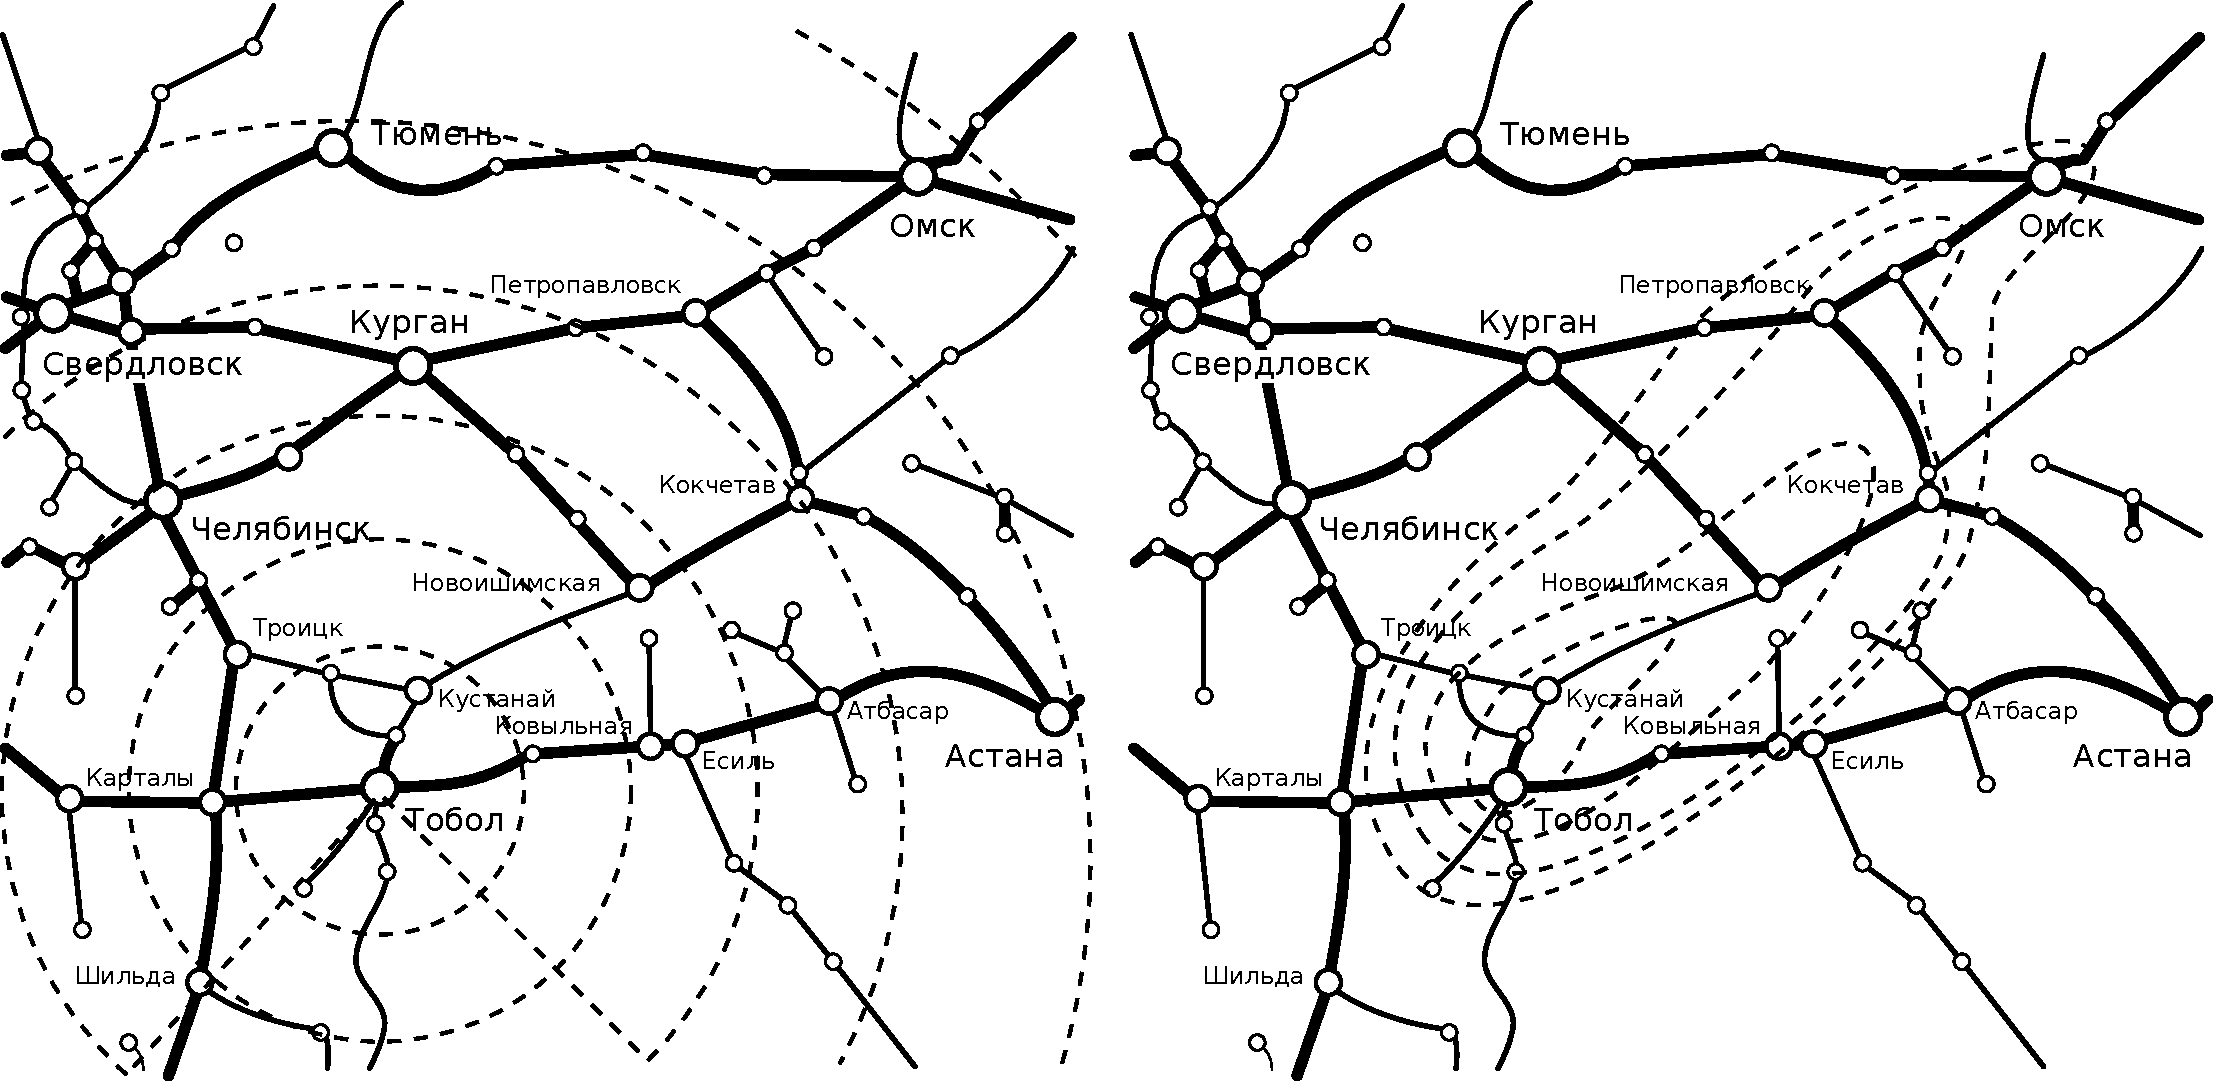
\includegraphics[width=\columnwidth]{yuzd1.pdf}
  \caption{Сужение области поиска}\label{fig:contraction}
% Исходник подложки.
% http://www.gdevagon.ru/scripts/info/map_old.php?X=C&Y=5
  %\label{fig:searchdescr}
\end{figure}

Зададим стоимость кротчайшего решающего пути, проходящий через некоторую вершину ГПС $x$, функцией $f:V\to R$ следующего вида:
\begin{equation}
  \label{eq:1}
  f(x)=g(x)+r(x),
\end{equation}
где $g(x)$~--- стоимость кратчайшего пути из начальной вершины до вершины $x$, а $r(x)$~--- стоимость пути из $x$ до целевой вершины.  Если $x$ является целевой вершиной то $r(x)=0$, и $g(x)=f(x)$, т.~е. значения функций равны стоимости решающего пути.  Если $x$ не является целевой, то значение $r(x)$ не известно.  Если значение $f(x)$ можно было бы вычислить для любой вершины $x$, то тогда можно было бы разработать алгоритм поиска, который точно <<знает>>, куда следует идти на каждом шаге построения решения.  Не смотря на то, что такое в общем случае невозможно, кое"=что все"=таки сделать можно: будем оценивать величину $r(x)$ снизу некоторой функцией $h(x)$.  Для всех $x$ должно выполняться $r(x)\leqslant h(x)$.  Значения функции $f(x)$ будем оценивать таким образом:
\begin{equation}
  \label{eq:2}
  f(x)\geqslant g(x)+h(x).
\end{equation}

В нашей задаче значения $h(x)$ соответствуют расстоянию между городами, т.е. по самой короткой линии на поверхности сферы.  Для вычисления этого расстояния нам потребуется база данных \texttt{geocache} (таблица~\ref{tab:dbstruct}) (о ней уже позаботились в разделе~\ref{sec:dbms}) и реализация подсистемы запроса географических координат на сервере \foreignlanguage{english}{OpenStreetMap}, которым в этот раз займемся чуть позже.

Программа поиска, основывающегося на оценке $h(x)$ состоит из трех основных предикатов.  Первый предикат~--- \texttt{after/6}, который получает еще два дополнительных параметра \texttt{GPS}~--- координаты целевой вершины (входной параметр), \texttt{F}~--- оценка $f(\mathtt{T})$ для вершины"=приемника \texttt{T} (выходной параметр).  Вторым предикатом выступает \texttt{bf1/3}, являющийся реализацией собственно алгоритма поиска.  Третий предикат~--- это процедура \texttt{bf/3}, предназначенная для подготовки данных для основного предиката \texttt{bf1/3}.

\begin{minted}{prolog}
bf1([_-s(G,[Target|T]) |_],         % (1)
        Target-_,s(G,[Target|T])):-!.
bf1([_-s(G,[X|T])|Ways], Target-GPS, S):-
        Target\=X,
        findall(F1-s(G1,[Y,X|T]),
           after([X|T],G,GPS, Y,G1,F1), L),
        append(L, Ways, NWays),
        keysort(NWays,SNWays),
        bf1(SNWays,Target-GPS,S).

after([S|R],SG, GPS, T,TG, F):-
        transdist(S,T,D),
        \+ member(T,[S|R]),
        TG is SG + D,
        geodist(T, GPS, GDist),     % (2)
        F is TG + GDist.

bf(Start, Target, Sol):-
        geocode(Target, Lon, Lat, _),
        bf1([0-s(0,[Start])],
          Target-ll(Lon,Lat), Sol). % (3)
\end{minted}


Используемые в программе структуры также немного усложнены по сравнению с UCS.  Элемент списка путей"=кандидатов (1) теперь представляет собой структуру вида \texttt{F-s(G,[X|T])}, где \texttt{X}~--- текущая вершина, \texttt{G}~--- стоимость пройденного пути $g(\mathtt{X})$ до текущей вершины, \texttt{F}~--- оценка $f(\mathtt{X})$.  Параметр \texttt{GPS} предиката \texttt{after/6}~--- структура \texttt{ll(Lon,Lat)}, \texttt{Lon}~--- долгота целевой вершины, \texttt{Lat}~--- ее широта.   Оба значения заданы в градусах.  Структура создается в строке (3) и передается в составе двойки \texttt{Target-GPS}.  Оценка $h(\mathtt{T})$ вычисляется в предикате \texttt{geodist/2} в строке (2).  Приведем пример запроса на поиск кратчайшего пути со станции \texttt{'Свердловск"=Сортировочный'} до станции \texttt{'Новосибирск"=Главный'}.

\begin{proexp}
?- bf('Свердловск-Сортировочный',
   'Новосибирск-Главный', S), write(S).
OSM: Пермь II
    lon: 56.1744706, lat:58.0050018    % (1)
S = s(1535,[Новосибирск-Главный,Обь,
    Татарская,Карбышево I,
    Войновка,Тюмень,Богданович,
    Шарташ,Свердловск-Сортировочный])
\end{proexp}


В результате запроса получается структура, которая содержит решающий путь и его стоимость (длина в км).  В процессе построения решения программа запрашивает данные местоположения станций в интернет.  Результаты запросов выдаются на экран в виде отладочной информации (1).

%\aaa{М.б. добавить какие-нибудь сравнения???} \aaa{Игра 15 хотя бы 1-2 примера. Но тогда надо добавлять описание задачи. }

Построенная нами реализация алгоритма $\mathtt{A}^*$ основывается на непереоценивающей функции $h$, т.е. выдает первым оптимальное решение.  Необходимо сделать пару замечаний.
\begin{enumerate}
\item Расстояние между городами вычисляется в пространстве на сфере, что не отражает структуры железнодорожной сети.  Например, расстояние между Москвой и Иркутском составляет чуть меньше 4200 км,  траектория полета самолета проходит вблизи города Сургут, находящийся достаточно далеко на север от Трассиба.
\item Запуская программу можно наблюдать, что гарантированно получить правильные координаты станции нам не всегда получится: сервис OSM не специализируется на предоставлении координат станций и может выдавать координаты объектов со схожим названием.  Так, например, на момент публикации данного пособия не удалось правильно определить координаты станции Лена, которая находится в городе Братске, Иркутской области.
\end{enumerate}
После небольшого экскурса в обработку файлов XML и доступа в интернет рассмотрим решение более общих задач на основе переборных алгоритмов.  \goforth{sec:britmuseum}


\subsection{Доступ в интернет и обработка XML}
\label{sec:inetxml}

Язык программирования Prolog представляет собой удобное средство обработки рекурсивных структур.  Использованные нами в разделе~\ref{sec:breadthfirst} списки относятся к таким рекурсивным структурам.  Другой известной рекурсивной структурой является \emph{дерево}, которое лежит в основе структуры формата данных XML (\foreignlanguage{english}{eXtensible Markup Language}) \cite{xml}.  Формат XML позволяет представлять информацию таким образом, чтобы она, с одной стороны, достаточно эффективно обрабатывалась алгоритмически (на компьютере), а с другой была понятна человеку.  Вот, например, ответ с сервера геокодирования \foreignlanguage{latin}{Nominatim} \cite{nominatim}:

\begin{minted}[fontsize=\footnotesize]{xml}
<?xml version="1.0" encoding="UTF-8" ?>
<searchresults timestamp='Thu, 15 Jan 15 07:54:30 +0000'
               attribution='Data © OpenStreetMap contributors, ODbL
                            1.0. http://www.openstreetmap.org/copyright'
               querystring='Иркутск'
               oviewbox='-112.15,61.44,112.15,-61.44'
               polygon='false'
               exclude_place_ids='158888259'
               >
  <place
      place_id='158888259' osm_type='relation' osm_id='1430614'
      place_rank='16'
      boundingbox="52.2094352,52.4217324,104.0579985,104.462928"
      lat='52.2895979' lon='104.2805843'
      display_name='Иркутск, городской округ Иркутск, Иркутская
                    область, Сибирский федеральный округ, Российская
                    Федерация'
      class='place' type='city' importance='0.70744217496694'/>
</searchresults>
\end{minted}


Основные элементы XML~--- это \emph{теги}, \emph{атрибуты} и текст, заполняющий пространство между тегами.  В данном примере тегами выступают \texttt{<searchresults>} и \texttt{<place>}.  Тег \texttt{<place>} расположен <<внутри>> тега \texttt{<searchresults>}.  Корневой тег (\texttt{<searchresults>}) по стандарту XML должен быть только один, остальные могут повторятся.  В нашем примере сервер геокодирования может выдать несколько объектов, соответствующих запросу.  В XML"=ответе сервера это отразится наличием повторений тега \texttt{<place>} для каждого объекта.

Атрибуты ассоциированы с тегами и несут формализованную дополнительную информацию.  В примере тегами \texttt{lat} и \texttt{lon} заданы географические координаты объекта (города Иркутска), полное наименование (\texttt{display\_name}), тип объекта \texttt{type} и т.~д.  Каждый атрибут приравнивается к некоторому значению.  Таким образом тег \texttt{place} со своими атрибутами описывает объекты, а \texttt{<searchresults>}~--- результат обработки запроса, состоящий из одного или нескольких объектов.

Реализация процедур (предикатов) обработки XML, запросы к сайтам интернет, а также обработка списка ключевых слов (атрибутов), реализованы в соответствующих библиотеках.  В нашей программе необходимо импортировать эти библиотеки.

\begin{proexp}
:- use_module(library(http/http_open)).
:- use_module(library(sgml)).   % Обработка XML
:- use_module(library(option)).
\end{proexp}


Предикат \texttt{geocodequery/4} запрашивает на сервере объекты по названию \texttt{Name} и возвращает широту, долготу и идентификатор объекта.  Библиотечная процедура \texttt{http\_open} в качестве первого аргумента принимает список ключевых слов в формате \texttt{<название структуры>(<значение>)}.  Элементы списка позволяют формировать строку URL запроса к серверу из отдельных компонент, что предоставляет удобный сервис для программиста.  Важным элементом этого списка является \texttt{search/1} со списком параметров запроса к скрипту \texttt{search.php}.  Параметр \texttt{format} указывает серверу тот факт, что ответ (перечень объектов) надо возвращать в виде XML.  Остальные значения понятны на интуитивном уровне.

Переменная \texttt{In} получает идентификатор входного потока данных, представляющих собой ответ сервера.  Этот поток передается в процедуру интерпретации XML как текста в XML, представленный в виде дерева (переменная \texttt{S}).  Переменная \texttt{S}, затем, унифицируется со структурой, представляющей собой шаблон внутреннего представления коревого тега.  Унификация помещает в \texttt{L} список тегов \texttt{<place>}.  Этот список анализируется в предикате \texttt{geoplace/4}, где изымается требуемые данные о местоположении найденных объектов.

\begin{minted}{prolog}
geocodequery(Name, Lon, Lat, ID):-
        http_open([
            host('nominatim.openstreetmap.org'),
            path('/search.php'),
            search([ q=Name,
                     lang=ru,
                     format=xml ])
            ], In, [] ),
        load_xml(In, S, []),
        S=[element(searchresults,_,[_|L])],
        close(In), geoplace(L, Lon,Lat,ID),
        writef("OSM: %w lon: %w, lat:%w",
                [Name, Lon, Lat]),nl.

geoplace(element(place,Attrs,_), Lon, Lat, Id):-
    option(lon(Lon1),Attrs), atom_number(Lon1,Lon),
    option(lat(Lat1),Attrs), atom_number(Lat1,Lat),
    option(place_id(Id),Attrs).
geoplace([X|_], Lon, Lat, Id):-
    geoplace(X, Lon, Lat, Id).
geoplace([_|T], Lon, Lat, Id):-
    geoplace(T, Lon, Lat, Id).
\end{minted}


Предикат \texttt{geoplace} в качестве первого параметра принимает структуру \texttt{element(place, <список атрибутов>, [])}, соответствующую тегу \texttt{place}, или список таких структур.  Предикат возвращает геоданные об объектах, представленных в списке тегов \texttt{place}.  Предикат \texttt{option(lon(Val),L)} ищет в списке \texttt{L} элемент вида \texttt{lon=Val} или \texttt{lon(Val)} и унифицирует соответствующим значением переменную \texttt{Val}.  Процедура \texttt{atom\_number(X,Y)} переводит атомы \texttt{X} (строки) в целые числа \texttt{Y} (и наоборот), если такое возможно.

Следующий текст представляет собой программу обеспечения доступа предикату \texttt{after/6} к геоданным по названию станции \texttt{Station}.

\begin{minted}{prolog}
geocode(Station, Lon, Lat, Id):-
    \+ number(Station),
    station(Station, _, Code, _),
    geocode(Code, Lon, Lat, Id).

geocode(Station, Lon, Lat, Id):-
    number(Station),
    geocache(Station, Lon, Lat, Id),!.

geocode(Station, Lon, Lat, Id):-
    number(Station),
    station(Name, _, Station, _),
    geocodequery(Name, Lon, Lat, Id),
    sqlite_query_f(db,
     'INSERT INTO geocache (station, lon, lat,
         place_id) values
         (%w,%w,%w,%w)'-[Station,Lon,Lat,Id],
    _),!.
\end{minted}


Сначала \texttt{geocode/4} пытается найти данные в локальной базе данных координат \texttt{geocache/4}.  Если попытка терпит неудачу, то осуществляется запрос к интернет"=сервису \foreignlanguage{latin}{Nominatim} и запись результата в базу данных \texttt{geocache} для дальнейшего использования.  В тексте SQL"=запроса \texttt{INSERT} \texttt{\%w} обозначает место вставки строкового представления очередного значения из списка \texttt{[Station,Lon,\ldots]}.  Предикат \texttt{sqlite\_query\_f/3} реализован в программе следующим образом.

\begin{minted}{prolog}
sqlite_query_f(Conn, S-Args, ROW):-
    swritef(Query, S, Args),
    sqlite_query(Conn, Query, ROW).
\end{minted}

Все преобразования из \texttt{\%w} в форматной строке \texttt{S} конкретные значения из списка \texttt{Args} занимается библиотечный предикат \texttt{swritef/3}.  Результат преобразования записывается в переменную \texttt{Query}.

Из приведенных примеров программного кода хорошо видно, что синтез двух реляционных языков программирования в рамках одного приложения производится достаточно просто, при этом не надо изобретать дополнительные конструкции, например, циклы по строкам результата запроса.  Поэтому разрабатывая в следующий раз информационную систему со встроенными подсистемами математического моделирования \cite{asya2008} следует задуматься над вопросом о том, где в ней будут использоваться императивные языки программирования, а какие подсистемы следует реализовать на реляционном языке программирования.

%\nnn{Можно сказать, что среда программирования Prolog вполне себе полноценный инструмент проектирования информационных систем.}


\chapter{Поиск решения на основе перебора} \label{sec:britmuseum}

Иногда приходится сталкиваться с задачами, эффективный алгоритм решения которых очевидным образом реализовать не удается, либо нет достаточно времени на анализ свойств задачи и поиск подходящего алгоритма. К таким задачам относятся, например, \emph{задачи с удовлетворением ограничений}\footnote{Англ. \emph{\foreignlanguage{english}{Constraint satisfaction problems}, CSP.}}. Такие задачи являются математическими проблемами, определенными на конечном наборе объектов, чьи значения должны удовлетворять ряду ограничений, выраженных в виде неравенств и логических выражений. Исследования в области решения задач CSP ведутся достаточно давно, и по сей день актуальность этих исследований только повышается.

К задачам CSP сводятся многие задачи искусственного интеллекта, в частности планирование действий. Задачи удовлетворения ограничений довольно часто демонстрируют большую комбинаторную сложность, и практически для каждой индивидуальной задачи строятся собственные варианты эвристических алгоритмов\footnote{Алгоритмов, где на этапах выбора очередного направления поиска решения из нескольких альтернатив используется дополнительная (по отношению к исходной) информация для задания этим альтернативам некоторого предпочтения.} их решения. Примеры известных задач~--- <<Восемь ферзей>>, <<Раскраска карты>>, <<Судоку>>, <<Поиск выполняющего набора>>, <<Составление расписания вуза>>.

Формально задачи CSP определяются следующим образом. Заданы вектор переменных $\vec{V}=\langle v_1, v_2, \ldots, v_n\rangle$, где $n$~--- количество переменных (натуральное); множество множеств $D=\{ d_1, d_2, \ldots,$ $d_n\}$, где $d_i$~--- непустое множество значений (домен), которые может принимать переменная $v_i$, $i=1,2,\ldots,n$. Задается также логическое условие $P(\vec{V})=P(v_1,v_2,\ldots,v_n)$, которое истинно, если значения, присвоенные переменным $v_i$, соответствуют условиям правильной комбинации. Например, для задачи <<Восемь ферзей>> $P(\vec{V})$ истинно, если все ферзи, расставленные на доске, не бьют друг друга. Иногда говорят о системе ограничений и о таких значениях переменных, при которых все ограничения выполняются (истинны). Систему ограничений можно записать как конъюнкцию индивидуальных ограничений, т.~е. свести опять же к единому логическому условию $P(\vec{V})$.

\subsection{Алгоритм <<Британского музея>>}

Одним из простых алгоритмов, решающих задачи CSP, является алгоритм <<Британского музея>>\footnote{В советской литературе вариант этого подхода известен как метод <<Отобразить и проверить>> (источник информации, к сожалению, потерян). В настоящее время широко используется термин <<Метод грубой силы>> (Brute Force Approach) для обозначения данного подхода.}. Алгоритм реализует самый общий подход в задачах поиска решения на основе последовательной проверки всех возможностей (одну за одной), начиная с самых простых решений.

Алгоритм реализует концептуальный, а не практический подход, оперируя огромным количеством возможных альтернатив. В частности, в теории он представляет способ найти самую короткую программу, которая решает конкретную задачу. Например, можно сгенерировать все возможные программы длиной в один символ. Проверить каждую программу, решает ли она эту задачу\footnote{Существует фундаментальная проблема остановки, которая делает такую проверку, в общем случае, невозможной.}. Если среди односимвольных программ не найдено программы, решающей задачу, перейти к просмотру программ длиной в два символа, затем в три и т.~д. В теории такой подход позволяет найти самую короткую программу, однако на практике такой перебор занимает недопустимо большое время вычислений (для многих задач больше, чем возраст Вселенной).

Название данный алгоритм получил ввиду высказывания Аллена Ньювэлла, Дж.~С. Шоу и Герберта А. Симона в 1958 году: <<... Вполне уместно предположить, что если посадить обезьян за печатные машинки, можно через некоторое время воспроизвести все книги в известном Британском музее>> в Лондоне.

Несмотря на всю идеалистичность подхода для задач небольшой размерности, алгоритм вполне пригоден. Для начала, конечно, нет необходимости порождать программы, достаточно порождать варианты значений переменных $v_i$, затем проверять выполнимость $P(\vec{V})$. Рассмотрим пример задачи.

\begin{example}
Разработать программу поиска списка счастливых билетов, состоящих из шести цифр. Подсчитать их количество.
\end{example}

\begin{minted}{prolog}
num(X) :- member(X, [0,1,2,3,4,5,6,7,8,9]).
gen([]).
gen([X|T]) :- num(X), gen(T).

p([A,B,C, D,E,F]) :-
        A + B + C =:= D + E + F.

lucky([A,B,C, D,E,F]) :-
        gen([A,B,C, D,E,F]),
        p([A,B,C, D,E,F]).
\end{minted}

Программа при помощи предиката \texttt{gen/1} порождает идентификаторы билетов. Предикат \texttt{p/1} проверяет, является ли билет счастливым. Процедура порождения списка счастливых билетов оформлена в виде предиката \texttt{lucky/1} и в комментариях не нуждается. Для запуска программы порождения списка надо выполнить команду:

\begin{proexp}
?- lucky(L).

L = [0,0,0,0,0,0] ? ;
L = [0,0,1,0,0,1] ? ;
L = [0,0,1,0,1,0] ? ;
L = [0,0,1,1,0,0] ? ;
L = [0,0,2,0,0,2] ?

yes.
\end{proexp}

\noindent{}Для подсчета количества счастливых билетов создадим еще одно вспомогательное правило:

\begin{minted}{prolog}
count(N) :- findall(Ticket, lucky(Ticket),
    Tickets), length(Tickets, N).
\end{minted}

\noindent{}Данное правило позволяет подсчитывать количество счастливых билетов, но не выводить их полный список на экран.

Выполним запрос (GNU-Prolog):

\begin{proexp}
?- count(N).
N = 55252

(630 ms) yes.
\end{proexp}

Приведенные программы являются также примерами использования стандартных \texttt{member/2} и \texttt{length/2} предикатов обработки списков.

\paragraph{Сужение области поиска.} Программа перебирает $10^6$ вариантов, из которых, как мы только что увидели, только около $5.5\cdot 10^4$ относятся к решению задачи. То есть примерно один из двадцати билетов~--- счастливый. Возникает вопрос: Можно ли усовершенствовать программу, чтобы уменьшить количество неправильных вариантов\footnote{Часто требуется как можно быстрее найти первое решение или самое короткое решение. В этом случае можно рассматривать и сокращение перебора и в области решений.} и сэкономить время решения задачи на проверке этих неправильных вариантов?

Первым делом давайте попробуем вычислить значение переменной \texttt{F is A+B+C-D-E}. Добавим к программе следующий код:

\begin{minted}{prolog}
lucky2([A,B,C, D,E,F]) :-
        gen([A,B,C, D,E]),
        F is A+B+C-D-E,
        num(F),
        p([A,B,C, D,E,F]).

count2(N) :- findall(Ticket, lucky2(Ticket),
        Tickets), length(Tickets, N).
\end{minted}

\begin{proexp}
?- count2(N).
N = 55252

(133 ms) yes.
\end{proexp}

Получено такое же количество решений, но за время в пять раз меньшее. Вычисленное значение \texttt{F} может быть отрицательным и больше 9, что противоречит условиям задачи, поэтому в новую процедуру порождения билетов необходимо добавить дополнительную проверку \texttt{num(F)}, которая выполняется, если \texttt{F} находится в требуемом диапазоне. Теперь порождается в 10 раз меньше билетов, даже с учетом тех, где \texttt{F} находится вне диапазона. То есть каждый второй сгенерированный билет~--- счастливый.  Если убрать уже ненужную повторную проверку \texttt{p/1}, то скорость исполнения программы увеличится еще на 30\,{}\% до 106 микросекунд, т.~е. уже более, чем в 6 раз быстрее первоначальной.

\begin{proexp}
?- count2(N).
N = 55252

(103 ms) yes.
\end{proexp}

\paragraph{Дополнительное ускорение.} Теперь попробуем найти \textbf{два} последних числа. Выражение \texttt{A+B+C-D} изменяется в пределах $-9,$ $-8,$ $\ldots,0,1,\ldots,26,27$: от \texttt{0+0+0-9} до \texttt{9+9+9-0}. Варианты, кода результат выражения~--- отрицательный заведомо, неподходящие, так же как если этот результат больше $18$, \texttt{9+9+9-9}. Можно еще усовершенствовать алгоритм, но оставим это в качестве упражнения. Теперь надо разработать подпрограммы, которые будут для диапазона $0,1,\ldots,18$. Будем решать просто отдельную переборную задачу: Задано число $S \in 0,1,\ldots,18$, найти два слагаемых \texttt{E} и \texttt{F}, дающих в сумме $N$. Дополним программу следующим кодом:

\begin{minted}{prolog}
lucky3([A,B,C, D,E,F]) :-
        gen([A,B,C, D]),
        S is A+B+C-D,
        S >= 0, S=<18,
        gen2(S, E,F).

count3(N) :- findall(Ticket, lucky3(Ticket),
        Tickets), length(Tickets, N).

gen2(0,0,0):-!.  % Выделим отдельно наглядные
gen2(18,9,9):-!. % тривиальные варианты.
gen2(N,A,B):-N<10, !, igen(N,A), B is N - A.
gen2(N,A,B):-D is N - 9, Z is 9 - D,
        igen(Z, A1), A is A1 + D, B is N - A.

% igen(N, A) для A порождает последовательности
% 0,1,2,...,N
igen(N, A) :- N>=1, M is N - 1, igen(M, A).
igen(N, N).
\end{minted}

\noindent{}Запускаем запрос:

\begin{proexp}
?- count3(N).
N = 55252

(47 ms) yes.
\end{proexp}


Теперь программа работает в 13 с лишним раз быстрее первоначальной и в 2 раза быстрее предыдущей, т.~е. примерно один из трех билетов не является счастливым. Конечно, программу можно совершенствовать дальше: перейти к порождению первых трех цифр, и, отталкиваясь от полученной суммы трех первых цифр, по аналогии с последним примером порождать соответствующие последовательности. Однако необходимо заметить, что программа\footnote{Авторы пособия не ставили целью найти эффективную и короткую программу для решения этой задачи. Задача~--- продемонстрировать ход рассуждений.} постепенно становится сложной, а текст все меньше и меньше воспринимаемым. Многие задачи требуют с каждым усовершенствованием увеличения программы в 2 раза для сокращения перебора ненужных вариантов также в 2 раза. Поэтому важно вовремя остановиться, либо искать какой"=либо новый подход.

\chapter{Компьютерная алгебра}
\label{cha:compalgebra}

Старшее поколение преподавателей"= и ученых"=математиков озабочена уровнем знаний студентов вузов в области высшей математики, особенно в части знаний оператора дифференцирования.  Студентам в некоторой степени препятствуют освоению популярных систем компьютерной алгебры.  По"=видимому здесь сказывается недостаточная практика в этом направлении.  Действительно, прежде, чем \emph{автоматизировать} некоторую \emph{творческую деятельность} необходимо детально в ней разобраться, и, самое главное, разбираться в случае необходимости.

Если не дают пользоваться существующими системами компьютерной алгебры, то предлагается разработать свою.  Заодно повторим базовые преобразования формул, реализуемые оператором дифференцирования.  В качестве побочного продукта получим навыки \emph{преобразования символьной информации}.

\section{Символьное дифференцирование}
\label{sec:}


Частную производную функции $f(x,y,\ldots)$ по переменной $x$ обозначают как
$$
f^{\prime}_x,\;f_x,\;\frac{\partial }{\partial x}f,\;\frac{\partial f}{\partial x}, \;\mbox{или}\; \frac{d_x f}{dx}.
$$
В языке Prolog обозначим частную производную предикатом \texttt{d(F,X,DF)}, где \texttt{F}~--- функция, производная \texttt{DF} которой <<берется>> по переменной \texttt{X}.  Программу нахождения производных из функций (выражений) начнем писать с самых простых вариантов: производной переменной, константы и атома.

\begin{minted}{prolog}
d(Y,X,1):-var(X),var(Y),
    Y==X,!.
d(Y,X,0):-
    var(Y),var(X),!.
d(C,_,0):-atomic(C),!.
\end{minted}

Предикат \texttt{==/2} позволяет определять не с одной ли той же переменной унифицированы \texttt{X} и \texttt{Y}.  Предикат \texttt{var/1} проверяет, является ли аргумент все еще переменной или нет.  Выполним тестовые запросы:

\begin{minted}{prolog}
?- d(X,X,D).      ?- X=Y,d(Y,X,D).
D = 1.            X = Y,
                  D = 1.
?- d(Y,X,D).
Y = A,            ?- d(1,X,D).
X = B,            D = 0.
D = 0.

?- d(a,X,D).
D = 0.
\end{minted}

Следующий этап~--- реализовать правила преобразования арифметических операций.

\begin{minted}{prolog}
d(U+V,X,DU+DV):-!,   d(U*V,X,DU*V+DV*U):-!,
        d(U,X,DU),           d(U,X,DU),
        d(V,X,DV).           d(V,X,DV).

d(U-V,X,DU-DV):-!,   d(U/V,X,(DU*V-DV*U)/(V^2)):-!,
        d(U,X,DU),           d(U,X,DU),
        d(V,X,DV).           d(V,X,DV).
\end{minted}

Теперь рассмотрим суперпозицию функций, формула является рекурсивной (цепной).
$$
\frac{\partial}{\partial x}f(g(x)) = \frac{\partial f}{\partial g}\frac{\partial g}{\partial x}.
$$
Соответствующее правило Prolog будет следующим:

\begin{minted}{prolog}
d(E,X, DExpF*DExp):-
    E=..[Atom, Exp],      % (1)
    atom(Atom),!,         % (2)
    d(Exp,X,DExp),        % (3)
    df(Atom, Exp, DExpF). % (4)
\end{minted}

Сначала надо удостовериться, что \texttt{E}~--- это функция.  Для этого попробуем представить \texttt{E} в виде списка \texttt{[Atom, Exp]} (1,2), где \texttt{Atom}~--- это название функции, а \texttt{Exp}~--- выражение (аргумент).  Затем в строке (3) производится построение производной из аргумента, а в (4)~--- обращение к набору правил соответствия функций выражениям"=производным.

\begin{minted}{prolog}
df(sin,E, cos(E)).
df(cos,E, -sin(E)).
df(ln,E, 1/E).
df(exp,E, exp(E)).
\end{minted}

Предикат \texttt{df(Fun,Exp, DExp)} переводит функцию \texttt{Fun} и ее аргумент \texttt{Exp} в выражение, представляющее производную \texttt{DExp}.  В этот список необходимо самостоятельно добавить другие известные функции.

Перейдем к дифференцированию конкретных выражений. Производная степенной функции, например, реализуется так:

\begin{minted}{prolog}
d(E^N,X, N*E^(N1)*DE):-!,
        d(E,X,DE),
        N1 is N-1.
\end{minted}

Проверим программу на нескольких выражениях:

\begin{proexp}
?- d(X^2, X, D).
D = 2*X^ (2-1)*1.

?- d(sin(X^2), X, D).
D = cos(X^2)* (2*X^ (2-1)*1).

?- d(sin(cos(X^2))*ln(X+Y), X, D).
D = cos(cos(X^2))* (-sin(X^2)*
    (2*X^ (2-1)*1))*ln(X+Y)+1/
    (X+Y)* (1+0)*sin(cos(X^2)).
\end{proexp}

Результат требует дальнейшего совершенствования~--- построение сокращенных выражений.  Для этого реализуем два набора правил: фасадный\footnote{Фасадный предикат предназначен для запуска пользователем.  За фасадом здания скрывается вся его сложная конструкция, доступная для понимания только специалистам. } предикат \texttt{sim/2}, предназначенный для сокращения выражений, и предикат \texttt{r/2}, представляющий собой элементарные упрощающие преобразования.  Если элементарное преобразование удалось, то \texttt{r/2} истинен, иначе он терпит неудачу.

\begin{minted}{prolog}
sim(X, X):-    % Переменная не сокращается.
    var(X),!.
sim(E, R):-    % Сделать один шаг упрощения.
    r(E,E1),!, % Если удалось, то
    sim(E1,R). % сократить результат еще.
sim(E,E).      % Выражение не сокращается.
\end{minted}

\noindent{}Реализация \texttt{sim/2} сильно походит на сортировку списка методом <<пузырька>> \cite{ais}.  Теперь рассмотрим правила элементарных преобразований.

\begin{minted}[texcomments]{prolog}
r(A+B, A):-B=@=0,!.  % A+0 $\to$ A
r(B+A, A):-B=@=0,!.  % 0+A $\to$ A
r(A*B, A):-B=@=1,!.  % A*1 $\to$ A
r(B*A, A):-B=@=1,!.  % 1*A $\to$ A
r(_*B, 0):-B=@=0,!.  % A*0 $\to$ 0
r(B*_, 0):-B=@=0,!.  % 0*A $\to$ 0
r(A^B, A):-B=@=1,!.  % $A^1$ $\to$ A
r(A^B, 1):-B=@=0,A\=@=0,!.  % (1)
r(A/B, A):-B=@=1,!.  % A/1 $\to$ A
r(B/A, A^(-1)):-B=@=1,!.    % (2)
\end{minted}

В строке (1) рассматривается случай $a^0=a$, исключая неопределенность $0^0=\frac{0}{0}$.  В строке (2) $\frac{1}{x}$ заменяется на $x^{-1}$.  В перечисленных правилах используется специальный вид унификации \texttt{=@=/2}, который проверяет структурную эквивалентность аргументов.  Представим несколько примеров\footnote{Специальные варианты унификаций SWI-Prolog рассматриваются на странице \url{http://www.swi-prolog.org/pldoc/man?section=unifyspecial}.} \cite{SWIP}:

\begin{minted}{prolog}
1    a =@= A    false
2    A =@= B    true
3    x(A,A) =@= x(B,C)  false
4    x(A,A) =@= x(B,B)  true
5    x(A,A) =@= x(A,B)  false
6    x(A,B) =@= x(C,D)  true
\end{minted}

Т.~е. с сокращаемых выражениях нам важно распознавать правильно где переменная, а где константа во входных параметрах.  Реализация первого правила \texttt{r/2} в виде

\begin{minted}{prolog}
r(A+0, A):-!.
\end{minted}

\noindent{}приводит к неправильному ответу на запрос\footnote{Последовательность слагаемых в запросе имеет принципиальное значение.}:

\begin{proexp}
?- r(2+X, R).
X = 0,
R = 2.
\end{proexp}

Автоматическая унификация Prolog по умолчанию при сопоставлении двух выражений подставляет переменные, символы, числа и другие термы вместо переменных в правое и в левое выражение так, чтобы они стали одинаковыми.  В данном примере овеществляется унификация \texttt{2+X=A+0}.  Если вместо \texttt{A} подставить \texttt{2}, а вместо \texttt{X}~--- \texttt{0}, то получим выражение \texttt{2+0=2+0}.  В нашем редукторе необходимо сокращаемые переменные сохранить как переменные \foreignlanguage{english}{Prolog}, чтобы потом можно было вычислять значения производных в точке.

\begin{minted}{prolog}
r(A+B, AB):-number(A),number(B),!,AB is A+B.
r(A*B, AB):-number(A),number(B),!,AB is A*B.
r(A+B, B+A):-number(B),!.
r(A*B, B*A):-number(B),!.

r(A+B+C,AB+C):-number(A),number(B),!, AB is A+B.
r(A*B*C,AB*C):-number(A),number(B),!, AB is A*B.
r(A+D, A+B+C):- \+ D=@=_, D=(B+C),!.
r(A*D, A*B*C):- \+ D=@=_, D=(B*C),!.
\end{minted}

Эти правила предназначены для переупорядочения слагаемых и сомножителей таким образом, чтобы можно было б сократить числовые выражения.  Два последних правила раскрывают <<ненужные скобки>>, перестраивая древовидное представление формулы.  Набор правил не полон, есть возможность их пополнить, в частности, можно алгоритмизировать операции вычитания и деления.  На самом деле цепочки последовательных операций сложения и вычитания, умножения и деления следует представить в виде списков слагаемых и сомножителей.  Затем надо производить упорядочение элементов этого списка согласно правилам представления полиномов, поиск и сокращение однородных членов.  Оставим эту задачу как упражнение.

Следующая группа правил пытается просто вычислить выражение, если такое возможно.  Если не получается вычислить, то попытаться сократить аргументы.

\begin{minted}{prolog}
r(E,R):-
    compound(E),
    ground(E),!,
    R is E.

r(E,R):-
    compound(E),
    E=..[F|Args],!,
    r(Args,SArgs),
    R=..[F|SArgs],
    E\=@=R.

r([],[]):-!.
r([X|T],[SX|ST]):-!,
    sim(X,SX),
    r(T,ST).
\end{minted}

Предикат \texttt{compound/1} проверяет, является ли его аргумент сложным выражением, а \texttt{ground/1}~--- выражением, не содержащим свободных переменных.  Первое правило, вообще говоря, реализовано некорректно: оно будет порождать исключительную ситуацию, если в выражении встретиться символ или список, т.е. что"=то, на чем невозможно выполнить арифметическую операцию.

Второе правило преобразует структуру к списку, аналогично тому, как мы делали с производной суперпозиции функции.  Затем производится сокращение выражений в аргументах функции.  В конце выражение собирается из отдельных компонент в результат сокращения.  Если получилась структура, отличная от исходной, то правило завершается удачно.

Последние два правила рекурсивно обрабатывают список аргументов.  Теперь рассмотрим пример использования компьютерной алгебры в программе расчета оптимального управления.

\section{Реализация численных методов оптимального управления}
\label{sec:optcontr}
\lstset{language=Python}

\newcommand{\vecx}{\mathbfit{x}}
%\newcommand{\vecx}{\vec{x}}
\newcommand{\vecf}{\mathbfit{f}}
\newcommand{\vecg}{\mathbfit{g}}
%\newcommand{\vecf}{\vec{f}}
\newcommand{\vecu}{\mathbfit{u}}
\newcommand{\vecpsi}{\mathbfit{\psi}}
\newcommand{\vecH}{\mathbfit{H}}

Разработка программ численного решения дифференциальных уравнений, расчеты оптимального управления связаны с необходимостью аналитических вычислений формул производных различных функций, и их реализации в виде программного кода.  В принципе, вместо реализации этого этапа разработки программ можно использовать численное дифференцирование и ограничиться только реализацией исходных функций.  Но как практически любой численный метод численное дифференцирование реализуется как а) итеративная процедура, которая затрачивает процессорное время на эти итерации; б) вносит погрешность вычисления, которая заложена уже в самом методе.  Использование аналитического вычисления производных в целом избавляет программный код от этих недостатков.

В \cite{pontr} рассмотрен метод вычисления оптимального управления, названного в честь его автора, академика Льва Семеновича Понтрягина, <<Принцип максимума Л.~С.~Понтрягина>>.  В книге вводится обозначение
$$
\vecpsi^T\vecx=\psi_ix^i=\psi_1x^1+\psi_1x^1+\ldots +\psi_nx^n,\quad i=1,2,\ldots,n;
$$
$$
\vecpsi=\vecpsi(t)=\left({\small
  \begin{array}{c}
    \psi_1,\\ \psi_2,\\ \vdots\\ \psi_n
  \end{array}}
\right),\qquad\vecx=\vecx(t)=\left({\small
  \begin{array}{c}
    x_1,\\ x_2,\\ \vdots\\ x_n
  \end{array}}
\right).\qquad
$$
В этом обозначении $x^1$~--- $i$-я фазовая переменная, $\vecpsi^T\vecx$~--- матричное произведение двух векторов, $\psi_ix^i$~--- скалярное произведение двух векторов.  Фазовые переменные описывают состояние некоторого объекта\footnote{Самолета, корабля, автомобиля, природного ресурса и т.~д.} (рис.~\ref{fig:phasecoords}) в пространстве, одна переменная~--- одна координата, составляющая вектора скорости и т.~п.  Фазовые переменные $x^i$~--- это вещественнозначные функции ($x^i\in\mathbb{R}$) времени $x^i(t)$.  Верхний индекс в именах переменных и функций используется здесь и далее ввиду того, что производные функций по переменным будут указываться в нижнем индексе.  Переменные $\psi_i=\psi_i(t)$~--- обобщение импульса, задающее влияние фазовой переменной $x^i(t)$ на управление в определенные моменты времени.  Вектор переменных $\vecx$ называется \emph{фазовым вектором} объекта (рис.~\ref{fig:phasecoords}), а вектора, аналогичные $\vecx(t)$,~--- \emph{вектор"=функциями}.

В фазовый вектор объекта входят его координаты и вектор скорости, а также другие физические величины, характеризующие состояние этого объекта в заданный момент времени $t\in[t_o,t_1]$.  На рис.~\ref{fig:phasecoords} изображен пример самолета и приведен его упрощенный фазовый вектор.  Переменные $x^1,x^2,\ldots,x^6$ задают его координаты и величины скоростей самолета по осям, $x^7,x^8$~--- угол рыскания и скорость его изменения.  Далее, аналогично $x^9,x^{10}$~--- угол горизонта, $x^{11},x^{12}$~--- угол крена, $x^{13}$~--- величина подъемной силы.  Переменная $x^{14}$ задает величину силы тяжести, $x^{15}$~--- величина сил, тормозящих самолет.

\begin{figure}[bh]
  \centering
  \footnotesize
      \def\xyz{$x^1,x^2,x^3,\;x^4,x^5,x^6$} \def\yaw{$x^7,x^8$} \def\pitch{$x^9,x^{10}$}
      \def\roll{$\!\!\!\!\!\!x^{11},x^{12}$} \def\lift{$x^{13}$} \def\down{$\!\!x^{14}$}
      \def\thrust{$u^1$} \def\rudder{$u^5$} \def\drag{$x^{15}$}
      \def\flaps{$u^2$} \def\aeleron{$u^3$} \def\engine{}
      \def\elevator{$u^4$} \def\svgwidth{0.80\columnwidth}
      \input{paropt/pics/Cessna-Plane.pdf_tex}
  \caption{Фазовый вектор самолета}
  \label{fig:phasecoords}
\end{figure}

Изменение переменных $\dot{x}^i(t)$ во времени в общем случае задается дифференциальным уравнением
\begin{equation}
  \label{eq:3}
\dot{x}^i=\frac{dx^i}{dt}=f^i(x^1,x^2,\ldots,x^n)=f^i(\vecx);\quad
   \dot{\vecx}=\frac{d\vecx}{dt}=\vecf(\vecx).
\end{equation}
При помощи этого уравнения задается, например, влияние геометрии оперения и силы тяги на вектор скорости самолета, влияние вектора скорости и силы тяжести на координаты в трехмерном пространстве и т.~п.  Дифференциальные связи второго порядка, например, влияние координаты объекта на величину силы тяжести также задаются при помощи уравнения (\ref{eq:3}) опосредованно при помощи системы из двух уравнения \cite{pontr}.

Система уравнений (\ref{eq:3}) определяет поведение объекта в процессе изменения времени.  В (\ref{eq:3}) вторая форма записи~--- векторная.  Задав $\vecx(t_0)=\vecx_0$ в момент времени $t_0$ и решив уравнение (\ref{eq:3}) можно рассчитать траекторию изменения объекта (перемещение его в пространстве, например), т.~е. решить задачу Коши.  Теперь обобщим уравнение (\ref{eq:3}), преобразуем его в следующий вид:
\begin{equation}
  \label{eq:4}
  \dot{\vecx}(t)=\vecf(t,\vecx(t),\vecu(t)),
\end{equation}
где $\vecu(t)$~--- \emph{управление}, которое также зависит от $t$.  Предполагается, что $\vecf(t)$ непрерывна по совокупности всех переменных и имеет непрерывные производные по каждому $x^i$ и $u^i$.

Как только в параметры $\vecf(t)$ добавили $\vecu(t)$ решение дифференциального уравнения (\ref{eq:4}) стало опять многозначным, т.~е. траектория зависит теперь не только от $\vecx_0$, но и от того как объектом управляют $\vecu(t)$.  На рис.~\ref{fig:phasecoords} в вектор управления $\vecu$ входят величина силы тяги $u^1$, а также $u^1,u^2,\ldots,u^5$, обозначающие величины сил, вызванных соответствующей геометрией крыла и хвостового оперения: закрылки, элероны, рули высоты и направления).  Геометрия крыла и хвостового оперения изменяется системой управления, например, человеком.  Далее будем предполагать, что самолетом управляет техническое устройство, например, компьютер с системой датчиков для получения значений элементов фазового ветра, а также выработанный им вектор $\vecu(t)$ каким"=либо образом меняет тягу и геометрию корпуса самолета.

Для того, чтобы <<выбрать>> из бесконечного количества возможных решений одно, необходимо из всех возможных траекторий выбрать в некотором смысле <<лучшую>>.  Какая траектория лучше, а какая хуже определяет функция"=критерий, отображающая траектории (или параметры, ее полностью определяющие) на некоторое число из $\mathbb{R}$.  В оптимальном управлении такая функция называется \emph{функционалом}.
\begin{equation}
  \label{eq:5}
  I(\vecx,\vecu)=\int\limits_{t_0}^{t_1}f^0(t,\vecx(t),\vecu(t))dt \to \min.
\end{equation}

В формуле (\ref{eq:5}) функция $f^0(t,\vecx(t),\vecu(t))$ вычисляет (формализует) значение критерия оценки качества траектории тела в момент времени $t\in[t_0,t_1]$, предполагается, что функция $f^0$ дифференцируема по переменным из $\vecx,\vecu$ (так же как и $\vecf$).  Значение функции $f^0$ в конечный момент времени $t_1$ не зависит от $\vecu(t)$, т.~к. в этот момент управлять\footnote{Переводить управляемый объект в новое стояние <<волевым усилием>> функции $\vecu.$} объектом уже не получиться.  В связи с этим перепишем функционал следующим образом:
\begin{equation}
  \label{eq:6}
  I(\vecx,\vecu)=\int\limits_{t_0}^{t_1}f^0(t,\vecx(t),\vecu(t))dt+F(t_1,\vecx(t_1)) \to \min.
\end{equation}

\noindent{}Теперь функция $F(t_1,\vecx(t_1))$ будет обозначать качество траектории в этот последний момент времени $t_1$, а интегральное выражение~--- на основную часть траектории, где объектом еще  управлять.

Принцип максимума определяется через функцию Гамильтона (Гамильтониан), которая имеет следующий вид:
\begin{equation}
  \label{eq:7}
  H(t,\vecx,\vecpsi,\vecu)=f^0(t,\vecx,\vecu)+\vecpsi^T\vecf(t,\vecx,\vecu).
\end{equation}

Управление $\vecu(t)$ будет оптимальным $\vecu^*(t)$ с соответствующей оптимальной траекторией $\vecx^*(t)$, если выполняется условие
\begin{equation}
  \label{eq:7}
  H(t,\vecx^*,\vecpsi,\vecu^*)\geqslant H(t,\vecx^*,\vecpsi,\vecu)
\end{equation}
для любого допустимого $\vecu(t)$.  Если привезти (\ref{eq:4})-(\ref{eq:7}) в одну систему и перепишем все уравнения через $H$, то получим следующую задачу оптимального управления \cite{sethi}:
\begin{equation}
  \label{eq:8}
  \left\{
    \begin{array}{ll}
      \dot{\vecx}=\vecH_{\vecpsi}, & \vecx(t_0)=\vecx_0,\\
      \dot{\vecpsi}=-\vecH_{\vecx}, & \vecpsi(t_1)=F(t_1,\vecx(t_1)).
    \end{array}
  \right.
\end{equation}
Т.~е. $\vecx(t)$ определяется своим левым $\vecx(t_0)$ концом, а $\vecpsi(t_1)$~--- правым.


\subsection{Дискретный вариант задачи улучшения управления}
\label{sec:discrete}

Использование численных расчетов предполагает постановку задачи в дискретном времени.  Для этого разобьем интервал $[t_0,t_1]$ на $N$ равных частей с шагом $h=(t_1-t_0)/N$, $N\in\mathbb{N}$.  Дискретные моменты времени можно обозначать $t_0,$ $t_0+h$, $t_0+2h,$\ldots, $t_1-h,$ $t_1$ или, как будет далее использовано в пособии $\t_0,$ $\t_1,$ $\t_2,$\ldots $t_j,$\ldots $\t_N$.  Функцию $\dot{\vecx}(t)$ в левой части (\ref{eq:4}) заменим на $\vecx(t_{j+1})$ и получим дискретный вариант уравнения движения следующего вида:
\begin{align}
  \label{eq:4d}
  &\vecx(t_{j+1})=\vecg(t_j,\vecx(t_j),\vecu(t_j)),\quad j\in\{0,1,\ldots,N\};\\
  \label{eq:4dcond}
  &\vecx(t_0)=\vecx_0, \quad \vecx(t)\in\mathbb{R}^n,  \quad \vecu(t)\in\mathbb{R}^m.
\end{align}
Формула (\ref{eq:4d}) уже не является дифференциальным уравнением, и преобразование из (\ref{eq:4}) в (\ref{eq:4d}) теперь задача пользователя нашей библиотеки.  Самый простой способ~--- применить простую схему интегрирования Эйлера:
\begin{equation}
  \label{eq:4d1} \nonumber
  \vecx(t_{j+1})=\vecx(t_j)+h\vecf(t_j,\vecx(t_j),\vecu(t_j)).
\end{equation}
Далее будем предполагать, что пользователь сам задает (\ref{eq:4d}).  Качество траекторий будем оценивать следующим функционалом:
\begin{equation}
  I(\vecx,\vecu)=\sum_{j=0}^{N-1}f^0(t_j,\vecx(t_J),\vecu(t_j))+F(t_N,\vecx(t_N)) \to \min.
    \label{eq103}
\end{equation}

Принцип максимума в данном дискретном случае определяется при помощи дискретного варианта функции Гамильтона
\begin{align}
  H(t_j,\vecx(t_j),\vecu(t_j))=&f^0(t_j,\vecx(t_j),\vecu(t_j))+\nonumber\\
   &\vecpsi^T(t_{j+1})\vecg(t_j,\vecx(t_j),\vecu(t_j)).   \label{eq:descH}
\end{align}

Выпишем теперь принцип максимума
\begin{align}
  H(t_j,\vecx^*(t_j),\vecpsi(t_{j+1}),\vecu^*(t_j))\geqslant H(t_j,\vecx^*(t_j),\vecpsi(t_{j+1}),\vecu(t_j)) \label{eq:descMax}
\end{align}
для всех допустимых $\vecu(t_j)$.  Сопряженная вектор"=функция $\vecpsi(t_j)$ вычисляется по схеме:
\begin{align}
  \label{eq:startPsi}
  \vecpsi^T(t_N)&=F_\vecx(t_N,\vecx(t_N)), \nonumber\\ \vecpsi^T(t_j)&=\vecpsi^T(t_{j+1})+\vecH_\vecx(t_j,\vecx^*(t_j),\vecpsi^T(t_{j+1}),\vecu^*(t_j)).
\end{align}

Так как условиям (\ref{eq:7}) и (\ref{eq:descMax}) соответствует минимум $I(\vecx,\vecu).$  Поиск минимума с использованием численного метода основывается на вычислении градиента $I\prime(\vecu)$ (по переменным $\vecu$).
\begin{align}
  I\prime(\vecu)&=\vecH_\vecu(t,\vecx(t),\vecpsi(t),\vecu(t)).
\end{align}

\subsection{Схема алгоритма улучшения первого порядка}
\label{sec:improvealg}
\def\H{\mathbfit{H}}
\def\x{\mathbfit{x}}
\def\u{\mathbfit{u}}
\def\f{\mathbfit{f}}
\def\F{\mathbfit{F}}
\def\bpsi{\mathbfit{\psi}}

Теперь мы знаем как вычислять градиент, используя эти знания, построим алгоритм улучшения $I(\vecx,\vecu)$.  Обозначим через $\langle\x^I(i),\u^I(i)\rangle$ некоторую допустимую траекторию и управление на всем отрезке времени $[t_0,t_1]$.  Цель шага улучшения~---  найти такую траекторию $\langle\x^{I\!I}(i),\u^{I\!I}(i)\rangle$, чтобы $I(\x^{I\!I},\u^{I\!I}) < I(\x^I,\u^I).$  Общая схема улучшения выглядит следующим образом:

\begin{enumerate}
 \item[1.] Задается начальное управление $\vecu^I(t)$, из уравнения \eqref{eq:4d} и условий \eqref{eq:4dcond} определяется $\vecx^I(t)$. Вычисляется $I(\vecx^I,\vecu^I).$
 \item[2.] Из системы $\mathbf{\psi}(t)=\vecH_\vecx,\;\bpsi(t_1)=-\F_\x,$ находим $\bpsi(t),$\\ где $\H(t,\x,\bpsi(t+h),\u)=\bpsi^{T}(t+h)\vecg(t,\x,\u)-f^{0}(t,\x,\u),$ производная $\vecH_\u$ находится в точке $\left(t,\x^{I}(t),\bpsi \left(t+h \right),\u^{I}(t)\right)$.
$$
\vecH_{\vecu}(t,\x,\bpsi(t+h),\u)=\vecg_{\vecu}(t,\x,\u)\bpsi(t+h)-f^{0}_\vecu(t,\x,\u),\mbox{из (\ref{eq:4dcond})}
$$
Задается параметр $\alpha$.
 \item[3.] Из системы $\x(t+h)=\vecg(t,\x(t),\u^{I\!I}(t)),$ $\x(t_0)=\x_0,$ где $\u^{I\!I}(t)=\u^{I}(t)+\alpha \H_\u,$ вычисляется $\x^{I\!I}(t).$
 \item[4.] Новое управление и значение параметра $\alpha$ подсчитываются из решения задачи одномерной минимизации для функционала $I(\x^{I\!I},\u^{I\!I})\to \min\limits_{\alpha}.$
 \item[5.] Если $I\left(\x^{I\!I},\u^{I\!I}\right)\geqslant I\left(\x^{I},\u^{I}\right)$ (улучшение не произошло), то уменьшаем $\alpha$ и переходим к следующей итерации, начиная с пункта~3.
 \item[6.] Иначе, если $I\left(\x^{I},\u^{I}\right)-I\left(\x^{I\!I},\u^{I\!I}\right)>\varepsilon$, то переходим к следующей итерации, начиная с пункта~2. Значение $\varepsilon$ --- параметр точности.
\end{enumerate}

Шестой шаг алгоритма не относится непосредственно к схеме улучшения, но он логичен, т.~к. создает итеративный процесс поиска минимума $I(\x,\u),$ т.~е. функции $\vecu$ оптимального  управления объектом.

\subsection{Реализация программы}
\label{sec:improprog}

Алгоритм реализуем на простом и компактном языке программирования Python \cite{pythondl,pythondoc,pythonbook}.  Язык является объектно"=ориентированным, его дистрибутив содержит огромное количество библиотек.  Кроме того, в интернете находится еще множество других библиотек и приложений, в том числе библиотеки \texttt{numpy} и \texttt{sympy}.  Библиотека \texttt{numpy} включает в себя операции с векторами данных и матрицами.  При помощи их будем задавать фазовый вектор, траектории, моменты времени, функцию управления и т.~п.  В библиотеке \texttt{sympy} содержатся операции вычисления производных из выражений, функции преобразования и сокращения выражений, а также процедуры преобразования выражений в байт"=код виртуальной машины Python (компиляции выражений в программный код).

Программу начнем реализовывать с импорта \texttt{numpy} и \texttt{sympy}, библиотеки специальных структур"=итераторов \texttt{itertools}, системной библиотеки \texttt{os}.
\begin{minted}{python}
import math
import numpy, sympy
import itertools
from sympy import symbols, diff, Symbol
import numpy.linalg
from sympy.utilities.lambdify import lambdify
import os

TupleType=type((1,))
ListType=type([])
\end{minted}

Сначала запрограммируем абстрактный класс, представляющий модель управляемого объекта.  В классе необходимо представить $\x_0$, определить размерности $n$ и $m$ вектор"=функций $\x$ и $\u$.  Вектор \texttt{U0} ($\u^{I}$) необходимо задать как начальное приближение синтезируемого управления.

\begin{minted}[texcomments]{python}
class Model(object):

    def __init__(self, X0, U0):
        self.X0=atleast_1d(X0)  # $\x_0$ должен быть вектором
        self.U0=U0
        self.N=self.X0.shape[0] # Размерность $\vecx$
        self.M=U0.shape[1]      # Размерность $\vecu$

    def F(self, x):
        return 0.0              # Заглушка по умолчанию

    def g(self, t, x, u):
        raise RuntimeError("метод реализуется в подклассе")

    def f0(self, t, x, u):
        return 0.0              # Заглушка по умолчанию
\end{minted}

Реализация схемы улучшения представляет собой класс \texttt{Process}, наследующий все свойства класса \texttt{VFCalc}, реализующего компьютерную алгебру над вектор"=функциями.  Реализацию \texttt{VFCalc} рассмотрим далее, а пока сосредоточимся на схеме улучшения.

Схема улучшения получает в качестве входных данных в конструктор \texttt{\_\_init\_\_} два параметра: \texttt{model}~--- класс"=потомок класса \texttt{Model} и \texttt{alpha}~--- параметр $\alpha$.  Для вычисления производных \texttt{VFCalc} необходимо знать размерности $\vecx$ и $\vecu$.  Конструктор также сохраняет функции $\vecf,$ $f$ и $F$ в виде специальных структур"=выражений \texttt{sympy}, над которыми можно производить операции дифференцирования.

\begin{minted}[texcomments]{python}
class Process(VFCalc):
    def __init__(self, model, alpha=1.0):
        VFCalc.__init__(self, model.N, model.M)
        t,x,u=self.v.t,self.v.x,self.v.u
        self.model=model; self.alpha=alpha
        self.v.g=model.g(t, x, u)    # Получить выражение $\vecg$
        self.v.f0=model.f0(t, x, u)  # Получить выражение $f^0$
        self.v.F=model.F(x)          # Получить выражение $F$

    def trajectory(self, U):         # Расчет траектории $\vecx(t)$
        x0=self.model.X0; X = [x0]   # по известному $\vecu$
        for t, u in enumerate(U):    # (0, u0), (1, u1)
            xn=self.model.g(t, X[t], u); X.append(xn)
        return array(X)

    def I(self, X, U):               # Вычисление $I(\vecx,\vecu)$
        def _a(acc, t):
            return acc + self.model.f0(t, X[t], U[t])
        return reduce(_a, range(len(X)-1), self.model.F(X[-1]))

    def optimize(self, t, eps=0.001, iters=1000): # Схема
        Up=self.model.U0             # $(\x^{I},\u^{I})$
        Xp=self.trajectory(Up)
        Ip=self.I(Xp,Up); it = 1     # $I(\x^{I},\u^{I})$
        while True:
            alpha = self.alpha
            Psi=self.Psi(t, Xp, Up)  # $\vecpsi(t)$
            _H_u=self.H((self.v.u,), t[:-1], Xp[:-1], Up, Psi)
            while True:
                _dU=_H_u*alpha       # $\vecH_\u\alpha$
                Un = Up + _dU
                Xn = self.trajectory(Un) # $(\x^{I\!I},\u^{I\!I})$
                In = self.I(Xn, Un)  # $I(\x^{I\!I},\u^{I\!I})$
                dI = Ip-In
                if abs(dI)<eps:      # Решение найдено
                    return In, Xn, Un, it, "opt"
                if iters<=0:         # Решение не найдено
                    return In, Xn, Un, it, "nonoptimal"
                iters-=1; it+=1
                if In>=Ip:
                    alpha/=2         # Новый параметр
                    continue         # шага улучшения
                else:
                    Xp, Up, Ip = Xn, Un, In
                    break
\end{minted}

В предыдущем отрезке программного кода переменные \texttt{X}, \texttt{U} и их аналоги~--- это массивы значений $\vecx(t)$ и $\vecu(t)$ для каждого момента времени $t$ на интервале $[t_0,t_1]$.

Вычисление $\vecpsi$ и нужной производной $\vecH$ реализуются при помощи специальных методов класса \texttt{Process}, которые описаны далее.  Операция \texttt{dot(A,B)} выполняет матричное умножение аргументов.  Если в качестве параметра этой операции передать два вектора"=строки, то второй вектор будет автоматически транспонирован в столбец.  Эта особенность реализации в библиотеке \texttt{numpy} позволяет тривиальные матричные умножения векторов делать без дополнительной явной операции транспонирования.  В результате операции \texttt{X[:-1]} возвращается последний <<\texttt{-1}>> элемент \texttt{X}, т.~е. $\x(t_1)$.

\begin{minted}[texcomments]{python}
    def Psi(self, t, X, U):
        v=self.v
        psie = -self.fun(v.F,(v.x,), t[-1], X[-1], U[-1])
        psi=[psie]; X=X[:-1]; t=t[:-1]
        _f0_x=self.fun(v.f0, (v.x,), t, X, U) # $f^0_\x$
        _g_x =self.fun(v.g, (v.x,), t, X, U)  # $\vecg_{\!\x}$
        j=len(t)-1; p=psie   # Начать с конца интервала
        while j>=1:
            i=t[j]; pp=p
            pn = dot(pp, _g_x[i]) - _f0_x[i]
            psi.append(pn); p=pn; j-=1
        psi=array(psi)
        return psi[::-1]     # Переставить в обратном порядке

    def H(self, vars, T, X, U, Psi):
        g=self.fun(self.v.g, vars, T, X, U)
        f0=-self.fun(self.v.f0, vars, T, X, U)
        H = alpha * f0
        for psi,_H,_g,i in zip(Psi, H, g, range(len(H))):
            _H += dot(psi,_g); H[i]=_H
        return H
\end{minted}

В приведенном отрезке кода в \texttt{H} передается список векторов переменных, по которым вычисляется производные $\vecH$, значения $\vecx$ и $\vecu$ на всем интервале времени, а также сам интервал времени и параметр $\alpha$.

Функции $\vecg,$ $f^0$ и $F$, задаваемые пользователем нашей библиотеки решения задач оптимального управления, в программе могут получить как значения в определенный момент времени (например, \texttt{X[:-1]}), так и на всем интервале (\texttt{X}).  Кроме того, формулы производных от $g^i$ могут <<вырождаться>> в константы, т.~е. \texttt{g} может выдать не вектор значений, когда это надо, а просто одно числовое значение.  Для того, чтобы меньше зависеть от этих случаев необходимо реализовать специальную функцию, которая возвращала бы адекватный по типу результат типу переданных ей параметров.  А вот внутри функции должно вычисляться значение нужной нам производной нужной нам функции.  Такой функцией в \texttt{Process} является \texttt{fun}.

\begin{minted}[texcomments]{python}
    def fun(self, f, vars, T, X, U):
        code,df=self.code(f, *vars) # Найти производную и скомпилировать ее.
        X=numpy.atleast_1d(X)       # Входной параметры X и U
        U=numpy.atleast_1d(U)       # должны быть векторами.
        if X.ndim>1:
            Xs=[X[:,i:i+1] for i in range(X.shape[1])]
            Us=[U[:,i:i+1] for i in range(U.shape[1])]
            args=(T,)+tuple(Xs+Us)
        else:
            args=(T,)+tuple(X)+tuple(U)
        rc=code(*args)  # Вычислить функцию (производную)
        rct=type(rc)
        rc=numpy.atleast_1d(rc)
        if type(T)==numpy.ndarray:
            try: # Попробовать транспонировать список
                if rct in [TupleType,ListType]:
                    rc=rc.reshape(rc.shape[:-1])
                    rc=rc.T
                    return rc
            except ValueError: pass # ... не получилось
            if T.shape[0]!=rc.shape[0]: # Константа $\to$ вектор
                nrc=numpy.zeros((len(T),)+rc.shape,dtype=float)
                nrc[:]=rc; rc=nrc
        return rc
\end{minted}

\subsection{Дифференцирование вектор"=функций}
\label{sec:VFdiff}

Теперь рассмотрим подсистему вычисления производных вектор"=функций.  Для этого разработаем специальный класс, экземпляры которого, настроены для поддержки нашей программы, реализующей схему улучшения.

Экземпляры прежде всего должны знать какого размера \texttt{N} фазовый вектор $\vecx$ и вектор управления $\vecu$ (\texttt{M}).  Эти параметры передаются в конструктор класса \texttt{VFCalc} при создании экземпляра.  Далее порождается ряд символов, специальных структур библиотеки \texttt{sympy}, обозначающих идентификаторы в выражениях.  При помощи этих символов записываются функции, из которых будут вычисляться производные.

Класс \texttt{VFCalc} кроме сервиса вычисления производных предоставляет возможности компиляции полученных выражений в байт"=код виртуальной машины среды исполнения \texttt{Python}.  Так как класс \texttt{VFCalc} является базовым для класса \texttt{Process} то его определение в тексте программы должно быть помещено перед определением \texttt{Process}.

\begin{minted}{python}
class Helper():
    pass

class VFCalc(object):
    def __init__(self, N,M):
        self.N=N; self.M=M; self.v=Helper()
        self.v.x=[Symbol('x'+str(i+1)) for i in range(self.N)]
        self.v.u=[Symbol('u'+str(i+1)) for i in range(self.M)]
        self.v.t=Symbol('t')  # Переменные для представления
                              #    выражений
    def diff1(self, f, var):  # Шаг вычисления производной
        if type(f) in [TupleType,ListType]:
            df=tuple([self.diff1(fi, var) for fi in f])
        else:
            df=tuple([diff(f, vi) for vi in var])
        if len(df)==1: df=df[0] # Лишние скобки
        return df

    def diff(self, f, *vars): # Производная вектор-функции
        cf=f
        for v in vars:        # Выполнить пошагово
            cf=self.diff1(cf, v)
        return cf

    def subs(self, f, s):     # Подстановка в вектор-функцию
        if type(f) not in [TupleType,ListType]:
            return f.subs(s)
        return tuple([self.subs(fi,s) for fi in f])

    def lambdify(self, f):    # Компилирование вектор-функции
        l=[self.v.t]          # Формирование списка
        l.extend(self.v.x)    #   параметров
        l.extend(self.v.u)
        fl=lambdify(l, f, "numpy") # Использовать арифметику
        return fl             #  из пакета numpy

    def code(self, f, *vars): # Вычислить производную
        df=self.diff(f, *vars)
        c=self.lambdify(df)   # и скомпилировать ее
        return c,df           # Возвратить оба результата
\end{minted}

Тестирование класса произведем при помощи следующего программного кода:

\begin{minted}{python}
d=VFCalc(2,2)
x1,x2=Symbol('x1'),Symbol('x2')
u1,u2=Symbol('u1'),Symbol('u2')
y1=x1**2*u1+x2*u2**2
y2=x1**2*x2**2*u1**2*u2**2
res=(d.diff([y1,y2],
    [x1,x2], [u1,u2]))
pprint (res)
return
\end{minted}

В приведенном коде \texttt{x1} и \texttt{x2}~--- переменные, формирующие вектор переменных $\vecx$, \texttt{u1} и \texttt{u2}~--- переменные, формирующие вектор переменных $\vecu$, функции \texttt{y1} и \texttt{y2} формируют вектор"=функцию $\vecf$, из которой берется производная $\vecf_{\vecx\vecu}$.  В результате получаем следующую матрицу функций:
\begin{minted}[style=bw]{python}
(((2*x1, 0), (0, 2*u2)),
 ((4*u1*u2**2*x1*x2**2,
   4*u1**2*u2*x1*x2**2),
  (4*u1*u2**2*x1**2*x2,
   4*u1**2*u2*x1**2*x2)))
\end{minted}

\subsection{Тестирование программы}
\label{sec:testing}

Тестирование программы проведем на простой модели.
\begin{align*}
  &g_1=x_1(t_j)+hu_1(t_j),\quad x_1(t_0)=1.0,\\
  &f^0=h(x_1^2+u_1^2),\quad F=0.0, \\
  &h=0.01,\quad t_0=0.0, t_i=t_0+h(i-1), t_N=t_1=1.0,\\
  &\vecu^I=0.0.
\end{align*}

Запрограммируем модель в виде класса, унаследовав его от \texttt{Model}.
\begin{minted}[texcomments]{python}
class LinModel1(Model):
    def __init__(self):
        X0=(1.0,)
        self.h = 0.01
        self.num = int((1.0-0.0) / self.h) # num=$N$
        self.T = linspace(start=0.0, stop=1.0, num=self.num)
        self.t = arange(len(self.T))  # 0,1,2,3,4,5...
        Model.__init__(self, X0=X0, U0=self.start_control())

    def start_control(self):  # $\vecu^I$=0.0
        U = [(0.0,) for t in self.t[:-1]]
        return array(U)

    def F(self, x):
        return 0.0

    def g(self, t, x, u):
        x0=x[0]; u0=u[0]
        return (x0+self.h*u0,)   # Схема Эйлера для $\dot{x_1}=u_1$.

    def f0(self, t, x, u):
        x0=x[0]; u0=u[0]
        return self.h * (x0*x0+u0*u0)
\end{minted}

Теперь создадим экземпляр задачи, передадим его в качестве параметра в процесс улучшения, который тоже экземпляр своего класса.  Проведем тестовый запуск.

\begin{minted}[texcomments]{python}
def test_1():
    m = LinModel1()          # Модель
    p1=Process(m, alpha=1.0) # Процесс улучшения
    iters=2000   # Максимальное количество итераций
    eps=0.001    # Точность аппроксимации минимума $I$
    rc=I1, X1, U1, it1, rstr =
        p1.optimize(m.t, eps=eps, iters=iters)
    print (I1, "iters:", it1)

test_1()         # Запуск теста
\end{minted}

В результате запуска вычислений получим результат следующего вида:
\begin{minted}{text}
0.776664425757 iters: 47.
\end{minted}
Получается, что за 47 итераций получено управление и траектория, оцениваемая минимальным функционалом со значением 0.777.  Траектория и управление выглядят изображены на рис.~\ref{fig:result}. На рисунке пунктирная линия~--- это синтезированное оптимальное управление, а непрерывная~--- траектория.
\begin{figure}[hb]
  \centering
  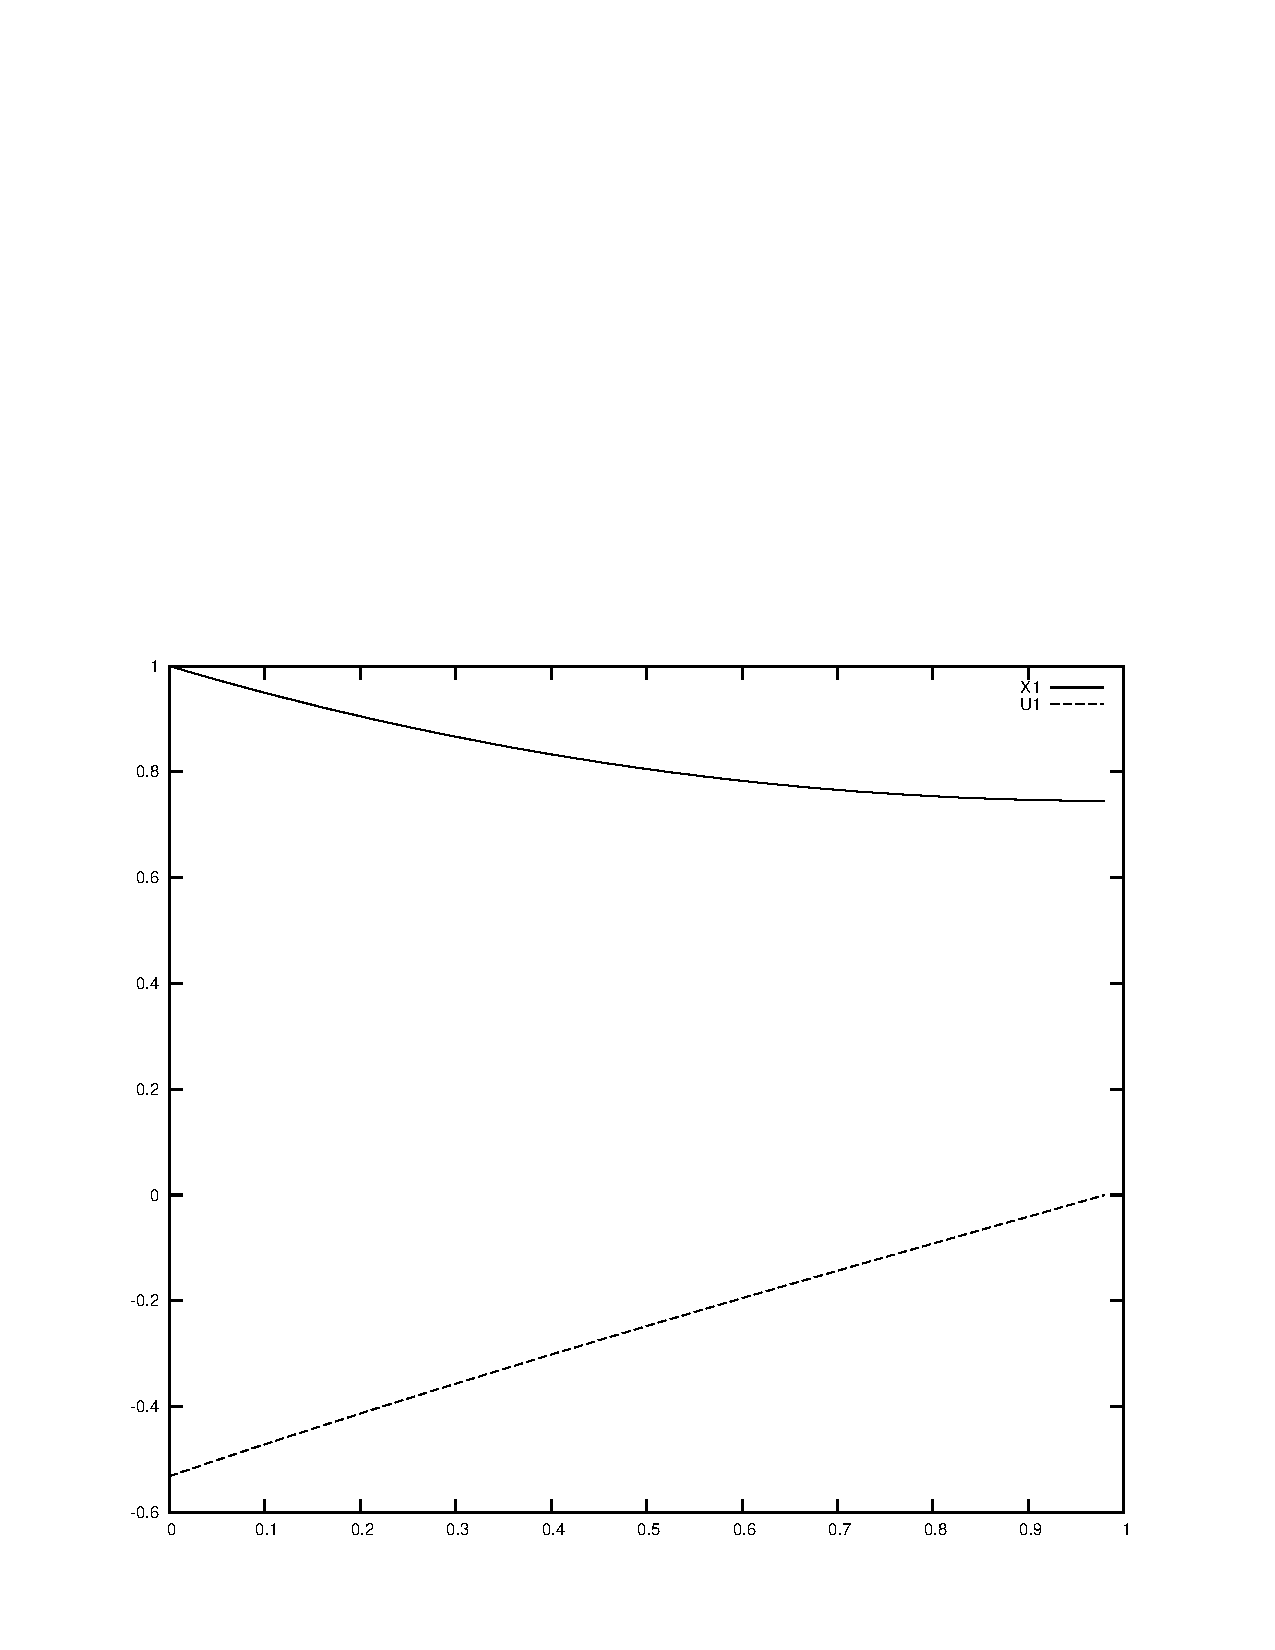
\includegraphics[width=0.7\linewidth]{my-plot}
  \caption{Результат расчета оптимального управления задачи}
  \label{fig:result}
\end{figure}


\subsection{Резюме}

В данной главе мы рассмотрели практическое приложение процедур вычисления частных производных из функций.  На самом деле данные процедуры не являются в полной мере реализациями какого"=либо метода искусственного интеллекта, но они демонстрируют как при помощи синтеза (гибридизации) численного моделирования и символьных вычислений возможно разрабатывать полезные приложения, а также экономить труд математиков и программистов: нет необходимости в выписывании и программировании процедур вычисления производных вектор"=функций.

Дальнейшим развитием изложенного подхода к разработке программного обеспечения численных методов является порождение программ, реализующих метод на основе анализа или интерпретации Python"=программы.  Интересным также является разработка библиотеки или программного пакета, при помощи которого можно было бы задавать уравнение движением в непрерывной форме вместе со схемой его перевода в дискретный вид для численного решения, а по полученной схеме опять же генерировать высокопроизводительную программу, реализация которой учитывает особенности микропроцессора.

% \section{Экспертные системы}
% \label{sec:es}

% \section{Управление вычислительным процессом}
% \label{sec:calcdss}


\chapter*{Заключение}

В учебном пособии приведены ряд задач искусственного интеллекта, решения которых представлены в виде программ на логическом языке программирования Prolog.  Задачи представлены классические, относящиеся к планированию действий, поиску решения с удовлетворением ограничений, так и апеллирующие к специфике численных методов решения дифференциальных уравнений и поиска оптимального управления движением.  Отдельно рассмотрено применение логического языка для организации символьных вычислений.  Свойства логического языка программирования позволяют программисту развить навыки логического мышления и отношению к своей программе не просто как к некоторому набору операторов, а как строгой логической конструкции.  Причем это касается не только языков программирования высокого уровня таких, как Prolog, Refal и языков функционального программирования, но и языков императивных: С/С++/С\#, Pascal, Visual Basic и т.д.

За рамками пособия остались такие интересные темы, как <<Эволюционные вычисления>>, <<Решение игровых задач>>, <<Экспертные системы>>, <<Анализ данных>> и др.

Надеемся, что задача пособия, рассказать на каких принципах работают совреммные системы компьютерной алгебры, выполнена, а студенты-читатаели с интересом знакомились с разделами пособия и выполняли задания.  Надеемся также, что тематика учебного пособия теперь будет представлять научный интерес читателей.

К сожалению, задачи, рассмотренные в пособии, всегда присутствуют в любом производственном процессе, связанным с обработкой информации, однако, эти задачи, как правило, остаются незамеченными.  Достаточно просто распознать вычислительную задачу, труднее~--- задачу, связанную с математическим моделированием, и совсем трудно~--- задачи автоматизации рассуждений и принятия решения.  Читателю следует и далее уделять некоторое время развитию навыков прграммирования систем искусственного интеллекта и анализу бизнес"=процессов предприятия и выявления этих необычных задач.

Успехов в изучении методов искусственного интеллекта!





%\listoffigures
%\addcontentsline{toc}{section}{Список иллюстраций}
%\listoftables
%\addcontentsline{toc}{section}{Список таблиц}
\begin{thebibliography}{99}\itemsep1pt \parskip 0pt plus 0.3pt
\bibitem{pontr} Понтрягин~Л.~С. Принцип максимума в оптимальном управлении. Изд.~2-е, стереотипное. М.\,: Едиториал УРСС,  2004.~--~64~с.
\bibitem{rzhddb} URL:\href{http://mapservis.ru/docs/tar_ruc_4.htm}{Тарифное руководство № 4. Книга 2. Часть 1. Алфавитный список железнодорожных станций.} [Электронный ресурс]\,{}: сайт. \url{http://mapservis.ru/docs/tar_ruc_4.htm} (дата обращения: 06.05.2015).
\bibitem{citycoords} \href{http://alextyurin.ru/?p=1037}{Географические координаты основных городов России}. [Электронный ресурс]\,{}: сайт. URL:\url{http://alextyurin.ru/?p=1037} (дата обращения: 06.05.2015).
\bibitem{Anderson} Андерсон~Р. \emphbib{Доказательство правильности программ}\,{}: пер. с англ.\,{}/ Р.~Андерсон. -- М.\,:\,Мир, 1982. -- 168~c.: ил.
\bibitem{Bratko} Братко~И. \emphbib{\href{http://royallib.ru/book/bratko_ivan/programmirovanie_na_yazike_prolog_dlya_iskusstvennogo_intellekta.html}{Программирование на языке ПРОЛОГ для искусственного интеллекта}}\,{}: пер. с англ.\,/ И.~Братко. -- М.\,:~Мир, 1990. -- 560~c.: ил.
\bibitem{Vass:2000} Васильев~С.~Н. \emphbib{\href{http://bookfi.org/book/616050}{Интеллектное управление динамическими системами}}\,{}/ С.~Н.~Васильев, А.~К.~Жерлов, Е.~А.~Федосов, Б.~Е.~Федунов. -- М.\,:~Физматлит, 2000. -- 352~с: ил.
\bibitem {AIDictionary} \emphbib{\href{http://aihandbook.intsys.org.ru/index.php/intro/ai-handbook}{Искусственный интеллект\,{}: в 3~кн.}}\,{}/ под ред. Э.~В. Попова. -- М.\,:~Радио и связь, 1990. -- 464 c.:\,{}ил.
\bibitem{Lauriere} Лорьер.~Ж.-Л.  \emphbib{\href{http://publ.lib.ru/ARCHIVES/L/LOR'ER_Jan_Lui/_Lor'er_J.L..html}{Системы искусственного интеллекта}\,{}: пер. с франц.}\,{}/ Ж.-Л. Лорьер. -- М.\,:~Мир, 1991. -- 568~с.: ил.
\bibitem{Malpas} Малпас~Дж. \emphbib{\href{http://padaread.com/?book=40731&pg=1}{Реляционный язык Пролог и его применение}}\,{}/ Дж.~Малпас. -- М.\,:~Наука, 1990. -- 464~с.
\bibitem{math_slov:88} \emphbib{\href{https://app.box.com/shared/793ukgvblxmj0hh6btw4}{Математический энциклопедический словарь}}\,{}/ гл.~ред. Ю.~В.~Прохоров. -- М.\,:~Сов.~энциклопедия, 1988. -- 847~c.
\bibitem{DDW} Непейвода~Н.~Н. \emphbib{\href{http://www.logic-books.info/taxonomy/term/215}{Прикладная логика\,{}: учеб. пособие}}\,{}/ Н.~Н.~Непейвода. -- 2-е изд. -- Новосибирск\,{}:~Изд-во Новосиб. ун-та, 2000. -- 521~c.: ил.
%\bibitem{DDWII} Непейвода~Н.~Н.  \emphbib{\href{http://philosophy.ru/library/logic_math/library/nepeivoda_prog.pdf}{Основания программирования}}\,{}/ Н.~Н.~Непейвода, И.~Н.~Скопин. -- Москва; Ижевск\,{}:~Институт компьютерных исследований, 2003 -- 880~c.: ил.
\bibitem {Russell} Рассел~С. \href{http://www.aiportal.ru/downloads/books/ai-modern-approach-2-edition-by-rassel-norvig.html}{Искусственный интеллект: современный подход}\,{}: пер. с англ.\,{}/ С.~Рассел, П.~Новриг. 2-е изд. -- М.\,:~Изд. дом <<Вильямс>>, 2006. -- 1408~c.: ил.
\bibitem{WIKI-DCG} \emphbib{\href{https://en.wikipedia.org/wiki/Definite_clause_grammar}{DC-грамматика}} [Электронный ресурс]\,{}// Wikipedia, The Free Encyclopedia\,{}: сайт. -- URL:\texttt{https://en.wikipedia.org/wiki/Definite\_clause\linebreak\_grammar}. (дата обращения: 28.11.2013).
\bibitem{GNUP} \emphbib{\href{http://www.gprolog.org/}{The GNU Prolog web site} [Электронный ресурс]\,{}: сайт}. URL:\url{http://www.gprolog.org/}. (дата обращения: 28.11.2013).
\bibitem{SWIP} \emphbib{\href{http://www.swi-prolog.org/}{SWI-Prolog's home} [Электронный ресурс]\,{}: сайт}. URL:\url{http://www.swi-prolog.org/}. (дата обращения: 28.11.2013).

\bibitem{pythondl} Welcome to Python.org.  [Электронный ресурс]\,{}: сайт. URL:\url{https://www.python.org/} (дата обращения: 11.01.2015).
\bibitem{pythondoc} \href{http://younglinux.info/sites/default/files/python_structured_programming.pdf}{Основы программирования на Python.}  [Электронный ресурс]\,{}: сайт. URL:\url{http://younglinux.info/sites/default/files/python_structured_programming.pdf}. (дата обращения: 11.01.2015).
\bibitem{pythonbook}М.~Лутц.  \href{https://vk.com/doc10903696_196246835?hash=4b80f3cf914c7d65dd&dl=f90686bee18e565271}{Изучаем Python, 4-е издание.}-- Пер.~с англ.--СПб.:Символ-Плюс, 2011. 1280~с.,~ил.
\bibitem{nominatim} OpenStreetMap Nominatim: Search.  [Электронный ресурс]\,{}: сайт. URL:\url{http://wiki.openstreetmap.org/wiki/Nominatim}. (дата обращения: 11.01.2015).
\bibitem{sethi}S.~P.~Sethi, G.~L.~Thomson. Optimal Control Theory: Applications to Management Science and Economics. 2nd Edition. 2005. 506~pp.
\end{thebibliography}
\label{lastpage}
\newpage
\thispagestyle{empty}
\mbox{}

\vfill\vfill\vfill\vfill

\hfill{}{\small\itshape Учебное издание}
\vspace{4ex}
\begin{center}
{\small\textbf{Черкашин} Евгений Александрович\\[1em]}
{\bfseries Компьютерные науки 4}\\[1em]
ISBN~978-5-9624-0938-2
\vfill

\small
Редактор \textit{Г.~А.~Борисова}\\
Верстка \textit{Е.~А.~Черкашин}

\vfill{}
{\small Макет подготовлен при помощи системы \LuaLaTeX\\\mbox{}}
\vfill{}

Темплан 2014\,{}г. Поз.\,{}186

\end{center}
\begin{center}\small
\noindent Подписано в печать 28.12.2013.
Формат~60$\times$90 1/16.\\  %Гарнитура \sutypeface{}.
%Верстка \LuaLaTeXe.
%Бумага офсетная. Печать офсетная. Усл.печ.л.
Уч.-изд.\,{}л.\,{}6,4. Усл.\,{}печ.\,{}л. 6,8. Тираж~100~экз. Заказ~170
\end{center}
\vspace{1ex}
\begin{center}\small
Издательство ИГУ\\{}
664003, г.\,{}Иркутск, бульвар Гагарина, 36
\end{center}
\end{document}

%%%%%%%%%%%%%%%%%%%%%%%%%%%%%%%%%%%%%%%%%%%%%%%%%%%

% Local Variables:
% TeX-parse-self: t
% TeX-auto-save: t
% TeX-master: t
% End:
